\section{Berechnung des Fahrtverlaufs}

Der Fahrtverlauf eines Fahrzeuges wird bei der Berechnung in zwei verschiedenen Arten gespeichert. Einmal in so genannten \textit{\$keyPoints}, welche in einem Array die Start- und Zielgeschwindigkeit (\textit{time\_0} und \textit{time\_0}), die Start- und Endposition (\textit{position\_0} und \textit{position\_1}) und die Start- und Endzeit (\textit{time\_0} und \textit{time\_1}) einer Beschleunigung bzw. Verzögerung abspeichern. Für die Überprüfung, ob ein Fahrzeug die zulässige Höchstgeschwindigkeit in einem Infrastrukturabschnitt überschreitet, für die spätere Übermittlung der Echtzeitdaten an das Fahrzeug und die exakte Positionsbestimmung, werden mittels der \textit{\$keyPoints} für jede Geschwindigkeitsänderungen (und bei konstanter Geschwindigkeit in 1 Meter Abständen) die aktuelle relative Position innerhalb eines Infrastrukturabschnitts, der Infrastrukturabschnitt, die aktuelle Zeit und die aktuelle Geschwindigkeit in einem Array gespeichert.
Der Fahrtverlauf wird mit der Funktion \textit{updateNextSpeed$($$)$} berechnet, welche als Parameter unter anderem die Zugdaten aus dem \textit{\$allUsedTrains}-Array, Start- und Endzeit der Fahrt (\textit{\$startTime} und \textit{\$endTime}), den Ziel-Infrastrukturabschnitt (\textit{\$targetSection}) und die relative Position in dem Ziel-Infrastrukturabschnitt (\textit{\$targetPosition}) übergeben bekommt.

Die für die Berechnung benötigten Daten werden in den in Tabelle \ref{table:vars} beschriebenen Variablen gespeichert.

\begin{table}
\begin{center}
\renewcommand{\arraystretch}{1.2}
\begin{tabular}{c|c}
Bezeichnung & Funktion \\ \hline
\textit{\$keyPoint} (Array)                   &   \makecell{Beschreibt eine Beschleunigung bzw. Verzögerung \\(\textit{position\_0}, \textit{position\_1}, \textit{time\_0}, \textit{time\_1}, \\ \textit{speed\_0}, \textit{speed\_1})}           \\ \hline
\textit{\$next\_section} (Array)                  &    IDs aller Abschnitte                  \\ \hline
\textit{\$next\_lenghts} (Array)                  &    Längen aller Abschnitte                  \\ \hline
\textit{\$next\_v\_max} (Array)                  &    Höchstgeschwindigkeit aller Abschnitte                  \\ \hline
\textit{\$indexCurrentSection} (Integer)                  &    Index des aktuellen Abschnitts               \\ \hline
\textit{\$indexTargetSection} (Integer)                  &    Index des Ziel-Abschnitts                  \\ \hline
\textit{\$cumulativeSectionLengthStart} (Array)                  &    Absolute Startposition aller Abschnitte                  \\ \hline
\textit{\$cumulativeSectionLengthEnd} (Array)                  &    Absolute Endposition aller Abschnitte                  \\ \hline
\textit{\$trainPositionChange} (Array)                  &    Alle absoluten Positionen des Fahrtverlaufs                  \\ \hline
\textit{\$trainSpeedChange} (Array)                  &   Alle Geschwindigkeiten des Fahrtverlaufs                  \\
\end{tabular}
\renewcommand{\arraystretch}{1}
\caption{Beschreibung der verwendeten Variablen für die Fahrtverlaufsberechnung}
\label{table:vars}
\end{center}
\end{table}

In dem folgenden Abschnitt werden die einzelnen Schritte beschrieben, die durchlaufen werden um den optimalen Fahrtverlauf zu berechnen. In der Darstellung ~\ref{fig:fahrtverlauf} wird der Ablauf grob schematisch dargestellt.

\begin{center}
\begin{figure}
\begin{tikzpicture}[node distance=1cm, auto,]
\node[punkt] (a) {Berechnung bei einer Beschleunigung auf die maximal mögliche Geschwindigkeit};
\node[below=of a, punkt] (b) {Wird die Geschwindigkeit in Infrastrukturabschnitten überschritten?};
\node[right=of b, punkt](c) {Neuberechnung unter Berücksichtigung der Geschwindigkeitsüberschreitung};
\node[below=of b, punkt] (d) {Wird die Mindestzeit auf einer Geschwindigkeit eingehalten?};
\node[right=of d, punkt](e) {Neuberechnung unter Berücksichtigung der Mindestzeit auf einer Geschwindigkeit};
\node[below=of d, punkt] (f) {Erreicht der Fahrzeug mit einer Verspätung das Ziel?};
\node[right=of f, punkt] (g) {Kann die Geschwindigkeit reduziert werden, ohne dass das Fahrzeug eine Verspätung hat?};
\node[below=of f, punkt] (h) {Übermittlung der Echtzeitdaten an das Fahrzeug};
\node[right=of g, punkt] (i) {Reduzierung der Geschwindigkeit unter Einhaltung der Ankunfrtszeit};

\draw [pil] (a) -- (b);
\draw [pil] (b) --  node[pos=0.5] {Ja} (c);
\draw [pil] (c.north) -- +(0,0.5) -|  (b.north); 
\draw [pil] (b) -- node[pos=0.5,left] {Nein} (d);
\draw [pil] (d) --  node[pos=0.5] {Nein} (e);
\draw [pil] (e.north) -- +(0,0.3) -|  (d.north); 
\draw [pil] (d) -- node[pos=0.5] {Ja} (f);
\draw [pil] (f) -- node[pos=0.5] {Ja} (g);
\draw [pil] (f) -- node[pos=0.5,left] {Nein} (h);
\draw [pil] (g) -- node[pos=0.5] {Ja} (i);
\draw [pil] (g.south) -- node[pos=0.5] {Nein} +(0,-1) |-  (h.east); 
\draw [pil] (i.south) -- +(0,-1) |-  (h.east); 
\end{tikzpicture}
\caption{Ablaufplan der Fahrtverlaufsberechnung}
\label{fig:fahrtverlauf}
\end{figure}
\end{center}

\subsection{Ermittlung der Start- und Endposition der einzelnen Infrastrukturabschnitte unter Berücksichtigung der Zuglänge}


Für die Berechnung eines exemplarischen Fahrtverlaufs wurden die in Tabelle \ref{table:infraex} definierten Infrastrukturabschnitte benutzt. Diese Abschnitte wurden so gewählt, sodass alle Funktionen und die Allgemeingültigkeit des Algorithmus gezeigt werden können und treten so im EBuEf nicht auf. 

\begin{table}
\begin{center}
\renewcommand{\arraystretch}{1.2}
\begin{tabular}{c| C{3cm} |c}
Infrastrukturabschnitts-ID & Länge & zulässige Höchstgeschwindigkeit \\ \hline
1000                   &   300 $m$    & 120 $km/h$                        \\ \hline
1001                  &    400 $m$   & 120 $km/h$                        \\ \hline
1002                   &   300 $m$    &        120 $km/h$                         \\ \hline
1003                   &    400 $m$   &         90 $km/h$                        \\ \hline
1004                   &    300 $m$   &            60 $km/h$                     \\ \hline
1005                   &   200 $m$    &           60 $km/h$                      \\ \hline
1006                   &  400 $m$     &      90 $km/h$                           \\ \hline
1007                   &  500 $m$     &      120 $km/h$                           \\ \hline
1008                   &   300 $m$    &      120 $km/h$                           \\ \hline
1009                   &   400 $m$    &      100 $km/h$                           \\ \hline
1010                   &   300 $m$    &      60 $km/h$                           \\ \hline
1011                   &   300 $m$    &         40 $km/h$                        \\ 
\end{tabular}
\renewcommand{\arraystretch}{1}
\caption{Exemplarische Infrastrukturabschnitte}
\label{table:infraex}
\end{center}
\end{table}

Als exemplarisch gewählte Zugdaten wurden die in Tabelle \ref{table:train-ex} definierten Daten verwendet.

\begin{table}[]
\begin{center}
\renewcommand{\arraystretch}{1.2}
\begin{tabular}{r L{3cm}}

relative Startposition                   &   10 $m$                         \\ 
relative Zielposition                  &    290 $m$                         \\ 
aktueller Infrastrukturabschnitt                   &   1001                         \\ 
Ziel-Infrastrukturabschnitt                  &    1010                         \\ 
Startgeschwindigkeit                   &   0 $km/h$                          \\ 
Zielgeschwindigkeit                   &    0 $km/h$                        \\ 
Zuglänge                   &    50 $m$                        \\ 
Bremsverzögerung                   &    0,8 $m/s^{2}$                        \\ 
Fahrplan vorhanden                   &    ja                        \\ 
Zeit bis zur nächsten Betriebsstelle                   &    210 $s$                        \\ 

\end{tabular}
\renewcommand{\arraystretch}{1}
\caption{Exemplarische Zugdaten}
\label{table:train-ex}
\end{center}
\end{table}

Die zuvor ermittelten nächsten Infrastrukturabschnitte inklusive derer Längen und zulässigen Höchstgeschwindigkeit müssen für die Berechnung des Fahrtverlaufs angepasst werden, da ein Fahrzeug erst beschleunigen darf, wenn das komplette Fahrzeug in den Infrastrukturabschnitt eingefahren ist. In Darstellung \ref{fig:it1} sind die Infrastrukturabschnitte dargestellt, so wie sie von dem Fahrzeug ermittelt wurden. Dabei werden alle Abschnitte, die das Fahrzeug schon durchfahren hat oder hinter dem Zielabschnitt liegen nicht dargestellt. Zudem wird in dem aktuellen Abshcnitt die relative Position von der Länge abgezogen und in der Zielabschnitt wird nur bis zur relativen Zielposition abgebildet. Dementsprechend ist der erste Abschnitt in der Darstellung \ref{fig:it1} der Abschnitt mit der ID 1001. Dieser hat aufgrund der aktuellen relativen Position des Fahrzeugs eine Länge von 290 $m$. Und der letzte Abschnitt ist der Abschnitt mit der ID 1010 und einer Länge von ebenfalls 290 $m$.

\begin{figure}
  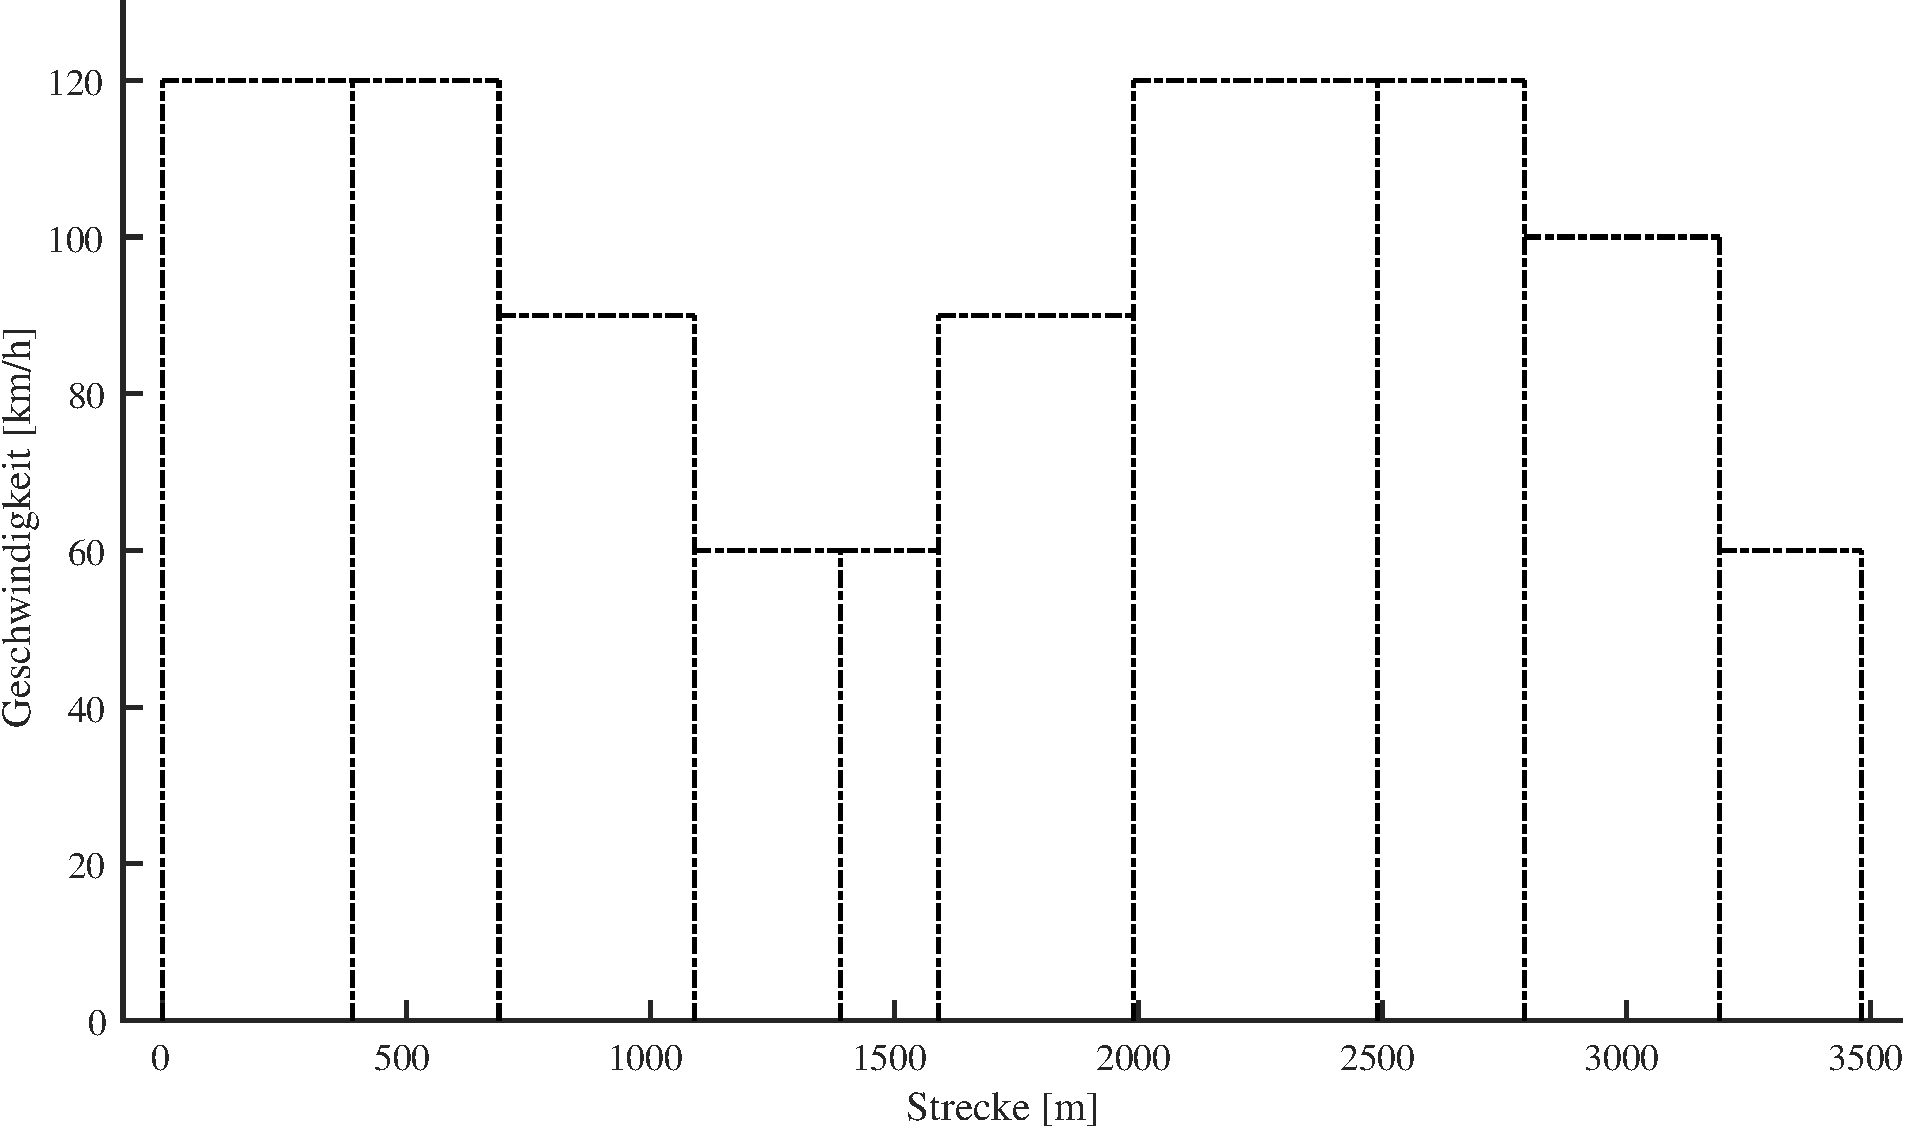
\includegraphics[width=\linewidth]{../matlab/it1.pdf}
  \caption{Darstellung der Infrastrukturabschnitte und die zugehörige Höchstgeschwindigkeit}
  \label{fig:it1}
\end{figure}

Bei der Berücksichtigung der Fahrzeuglänge wird durch alle Infrastrukturabschnitt iteriert und die Zuglänge auf die Länge das Abschnitts addiert. Von dieser neu ermittelten Endposition des Abschnitts wird überprüft, ob zwischen der vorherigen Endposition und der neu ermittelten Endposition ein Infrastrukturabschnitt liegt, dessen zulässige Höchstgeschwindigkeit geringer ist, als die des ursprünglichen Abschnitts. Wenn dieser Fall eintritt, wird der Abschnitt nur so weit verlängert, sodass keine Höchstgeschwindigkeit der folgenden Abschnitte überschritten wird. Von der neu ermittelten Endposition wird überprüft, in welchem Abschnitt diese liegt und mit dem Abschnitt wird dann weiter gerechnet. Sobald der Ziel-Abschnitt erreicht wurde, wird die Schleife abgebrochen. Die neu ermittelten Abschnitte werden in den Arrays \textit{\$next\_lengths\_mod} und \textit{\$next\_v\_max\_mod} abgespeichert. Durch diese Algorithmus kann es dazu kommen, dass sich die Anzahl der Abschnitte verändert hat. Dementsprechend können die Abschnitte nicht mehr eindeutig mit der Infrastruktur-ID bezeichnet werden. Mittels \textit{\$next\_lengths\_mod} und \textit{\$next\_v\_max\_mod} werden mit der Funktion \textit{createCumulativeSections$($$)$} für jeden Abschnitt die absolute Start- und Endposition in den Arrays \textit{\$cumulativeSectionLengthStartMod} und \textit{\$cumulativeSectionLengthEndMod} gespeichert. Diese Umwandlung ist essentiell für die Überprüfung, in welchem Abschnitt ein Fahrzeug sich aktuell befindet. Die neu berechneten Abschnitte werden sind in der Darstellung \ref{fig:it2} in rot abgebildet und beschreiben die maximale Geschwindigkeit, die ein Fahrzeug fahren darf an der jeweiligen Position.

\begin{figure}
  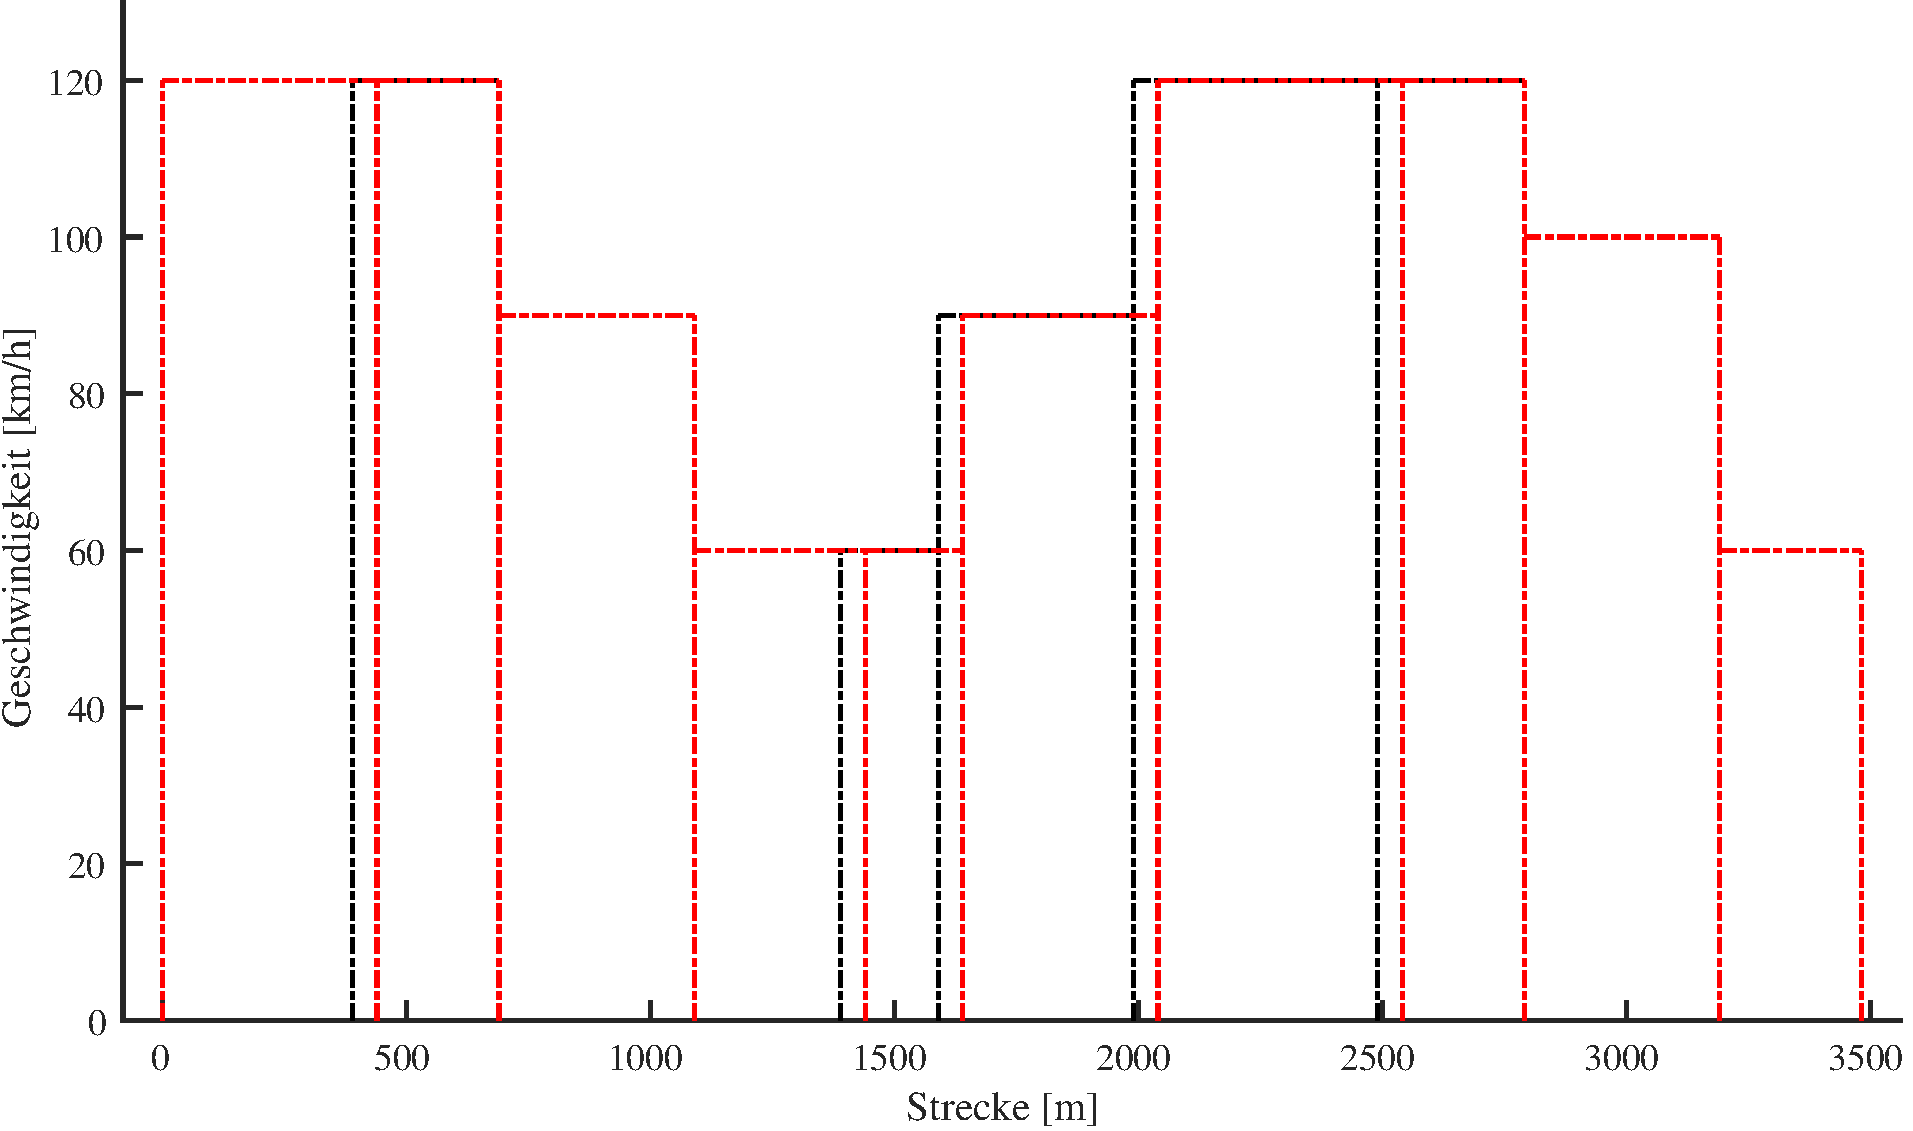
\includegraphics[width=\linewidth]{../matlab/it2.pdf}
  \caption{Darstellung Infrastrukturabschnitte und die zugehörige Höchstgeschwindigkeit unter Berücksichtigung der Fahrzeuglänge}
  \label{fig:it2}
\end{figure}

\subsection{Berechnung bei einer Beschleunigung auf die maximal mögliche Geschwindigkeit} \label{v_max}

Im ersten Schritt für die Distanz zwischen der aktuellen Position und der Ziel-Position mittels \textit{\$cumulativeSectionLengthStart}, \textit{\$cumulativeSectionLengthEnd}, \textit{\$indexCurrentSection} und \textit{\$indexTargetSection} berechnet. Für diese Distanz und die Startgeschwindigkeit wird mit Hilfe der Funktion \textit{getVMaxBetweenTwoPoints$($$)$} (Code-Beispiel ~\ref{lst:getVMaxBetweenTwoPoints}) die maximale Geschwindigkeit ermittelt, die das Fahrzeug aufnehmen kann, um noch bis zum Ziel rechtzeitig bremsen zu können. Dabei wird in 10 $km/h$-Schritten iteriert und der maximale Wert zurückgegeben. Innerhalb der Funktion wir die Funktion \textit{getBrakeDistance$($$)$} (Code-Beispiel ~\ref{lst:getBrakeDistance}) aufgerufen, welche die benötigte Distanz für eine Beschleunigung bzw. Verzögerung berechnet. 

\begin{figure}
\begin{lstlisting}[caption={\textit{getVMaxBetweenTwoPoints$($$)$}},captionpos=b,label={lst:getVMaxBetweenTwoPoints}]
function getVMaxBetweenTwoPoints(float $distance, int $v_0, int $v_1) {
	global $verzoegerung;
	global $globalFloatingPointNumbersRoundingError;

	$v_max = array();
	for ($i = 0; $i <= 120; $i = $i + 10) {
		if ((getBrakeDistance($v_0, $i, $verzoegerung) + getBrakeDistance($i, $v_1, $verzoegerung)) < ($distance + $globalFloatingPointNumbersRoundingError)) {
			array_push($v_max, $i);
		}
	}
	if (sizeof($v_max) == 0) {
		if ($v_0 == 0 && $v_1 == 0 && $distance > 0) {
			echo "Der zug müsste langsamer als 10 km/h fahren, um das Ziel zu erreichen.";
		} else {
			// TODO: Notbremsung
		}
	} else {
		if ($v_0 == $v_1 && max($v_max) < $v_0) {
			$v_max = array($v_0);
		}
	}
	return max($v_max);
}
\end{lstlisting}
\end{figure}

\begin{figure}
\begin{lstlisting}[caption={\textit{getBrakeDistance$($$)$}},captionpos=b,label={lst:getBrakeDistance}]
function getBrakeDistance (float $v_0, float $v_1, float $verzoegerung) {
	if ($v_0 > $v_1) {
		return $bremsweg = 0.5 * ((pow($v_0/3.6,2)-pow($v_1/3.6, 2))/($verzoegerung));
	} if ($v_0 < $v_1) {
		return $bremsweg = -0.5 * ((pow($v_0/3.6,2)-pow($v_1/3.6, 2))/($verzoegerung));
	} else {
		return 0;
	}
}
\end{lstlisting}
\end{figure}

Durch die gegebene Startgeschwindigkeit und die höchstmögliche Geschwindigkeit wird ein erster Fahrtverlauf berechnet. Dabei werden zwei \textit{\$keyPoints} erzeugt. Mithilfe der Funktion \textit{createTrainChanges$($$)$} wird aus diesen beiden \textit{\$keyPoints} für jede Geschwindigkeitsveränderung die aktuelle absolute Position und Geschwindigkeit ermittelt. An den Positionen, an den das Fahrzeug eine konstante Geschwindigkeit hat, wird in 1 Meter Abständen die absolute Position und die Geschwindigkeit gespeichert. Die ermittelten Daten werden in den Arrays \textit{\$trainPositionChange} und \textit{\$trainSpeedChange} gespeichert. In der Darstellung \ref{fig:it3} ist das Ergebnis der 1. Iteration abgebildet.

\begin{figure}
  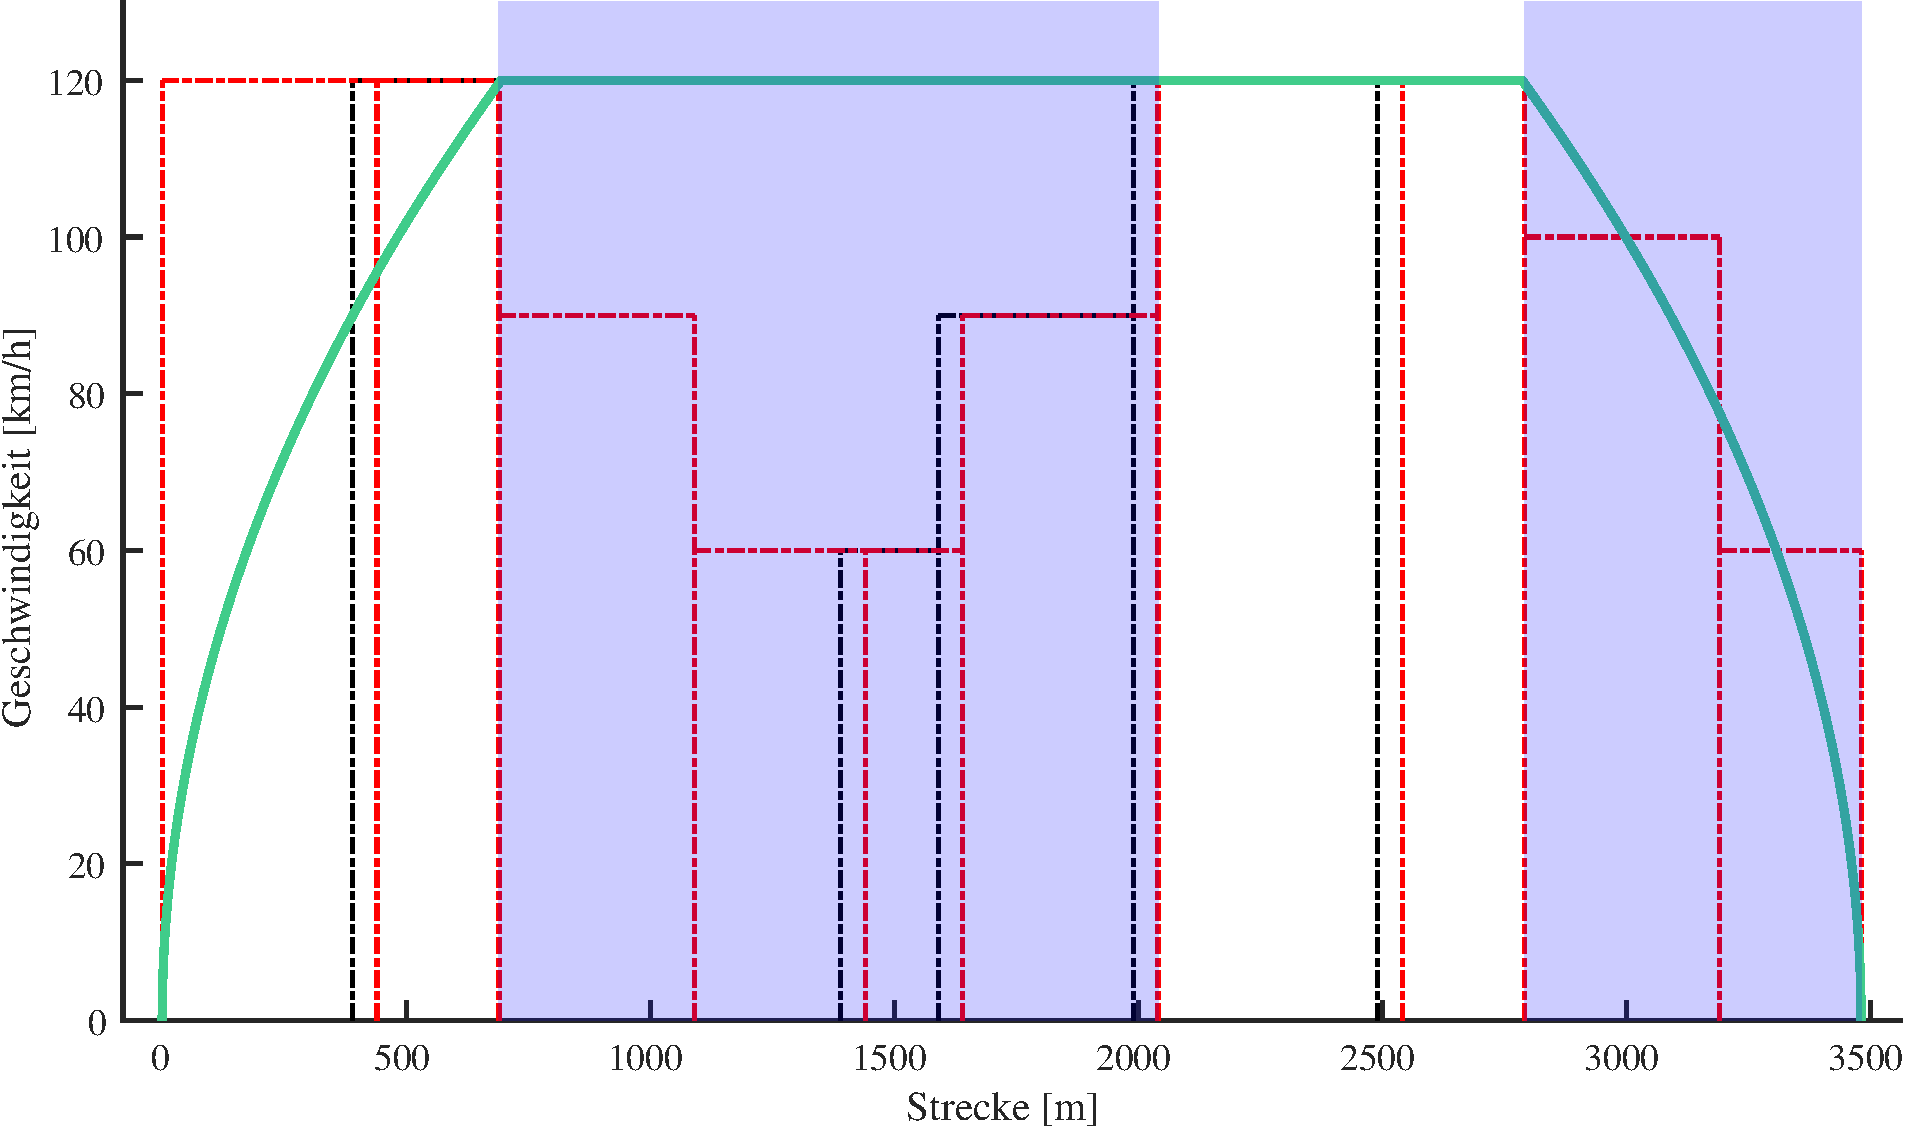
\includegraphics[width=\linewidth]{../matlab/it3.pdf}
  \caption{Fahrtverlaufberechnung (1. Iteration)}
  \label{fig:it3}
\end{figure}

\subsection{Überprüfung des Fahrtverlaufs nach Geschwindigkeitsüberschreitungen} \label{überprüfung}

Für die Überprüfung, ob bei einem Fahrtverlauf in manchen Infrastrukturabschnitten die zulässige Höchstgeschwindigkeit überschritten wird, wird nach jeder Berechnung die Funktion \textit{checkIfTrainIsToFastInCertainSections$($$)$} (Code-Beispiel ~\ref{lst:checkIfTrainIsToFastInCertainSections}) aufgerufen. In dieser Funktion wird über alle absoluten Positionen (\textit{\$trainPositionChange}) iteriert, überprüft in welchem Abschnitt sich diese Position befindet und überprüft, ob die zugehörige Geschwindigkeit aus dem \textit{\$trainSpeedChange}-Array die zulässige Höchstgeschwindigkeit überschreitet. Sobald in einem Abschnitt eine Geschwindigkeitsüberschreitung vorliegt, wird der zugehörige Index des Abschnitts in dem \textit{\$faildSections}-Array gespeichert. Diese Abschnitte sind in der Darstellung \ref{fig:it3} Lila hinterlegt. Als Rückgabewert der Funktion wird wird ein Array wiedergegeben, welches abspeichert, ob es zu einer Geschwindigkeitsüberschreitung gekommen ist (\textit{\grqq{}failed\grqq{}}) und wenn das der Fall ist auch die Indexe der Abschnitte (\textit{\grqq{}failed\_sections\grqq{}}).

\begin{figure}
\begin{lstlisting}[caption={\textit{checkIfTrainIsToFastInCertainSections$($$)$}},captionpos=b,label={lst:checkIfTrainIsToFastInCertainSections}]
function checkIfTrainIsToFastInCertainSections() {
	global $trainPositionChange;
	global $trainSpeedChange;
	global $cumulativeSectionLengthStartMod;
	global $next_v_max_mod;
	global $indexTargetSectionMod;

	$faildSections = array();

	foreach ($trainPositionChange as $trainPositionChangeKey => $trainPositionChangeValue) {
		foreach ($cumulativeSectionLengthStartMod as $cumulativeSectionLengthStartKey => $cumulativeSectionLengthStartValue) {
			if ($trainPositionChangeValue < $cumulativeSectionLengthStartValue) {
				if ($trainSpeedChange[$trainPositionChangeKey] > $next_v_max_mod[$cumulativeSectionLengthStartKey - 1]) {
					array_push($faildSections, ($cumulativeSectionLengthStartKey -1));
				}
				break;
			} else if ($cumulativeSectionLengthStartKey == $indexTargetSectionMod) {
				if ($trainPositionChangeValue > $cumulativeSectionLengthStartValue) {
					if ($trainSpeedChange[$trainPositionChangeKey] > $next_v_max_mod[$cumulativeSectionLengthStartKey]) {
						array_push($faildSections, $cumulativeSectionLengthStartKey);
					}
					break;
				}
			}
		}
	}

	if (sizeof($faildSections) == 0) {
		return array("failed" => false);
	} else {
		return array("failed" => true, "failed_sections" => array_unique($faildSections));
	}
}
\end{lstlisting}
\end{figure}

\subsection{Neuberechnung unter Berücksichtigung der\\Geschwindigkeitsüberschreitung}  \label{neuberechnung}

In dem Fall, dass es zu einer Geschwindigkeitsüberschreitung gekommen ist, wird der Fahrtverlauf neu berechnet. Als Grundlage dafür diesen die \textit{\grqq{}failed\_sections\grqq{}} aus der \textit{checkIfTrain\\IsToFastInCertainSections$($$)$} Funktion (Code-Beispiel ~\ref{lst:checkIfTrainIsToFastInCertainSections}). Die Funktion \textit{recalculateKeyPoints$($$)$} vergleicht immer zwei benachbarte \textit{\$keyPoints} und berechnet in dem Fall einer Geschwindigkeitsüberschreitung mit der Funktion \textit{checkBetweenTwoKeyPoints$($$)$} diese neu. In dem Fall, dass zwischen zwei benachbarten \textit{\$keyPoints} die zulässige Höchstgeschwindigkeit überschritten wird, wird die absolute Start- und End-Position dieser Geschwindigkeitsüberschreitung gespeichert. Im folgenden Schritt wird wie in dem Abschnitt \ref{v_max} zwischen den Start-Werten des ersten \textit{\$keyPoints} und der ersten Geschwindigkeitsüberschreitung die maximale Geschwindigkeit berechnet und zwei neue \textit{\$keyPoints} erzeugt. Das gleiche passiert zwischen der Position der letzten Geschwindigkeitsüberschreitung und den End-Werten des zweiten \textit{\$keyPoints}. Dadurch wird sichergestellt, dass es immer eine gerade anzahl an \textit{\$keyPoints} gibt und somit in jedem Iterationsschritt zwei benachbarte \textit{\$keyPoints} verglichen werden können. Nachdem alle \textit{\$keyPoint}-Paare überprüft werden, werden mit Hilfe der \textit{createTrainChanges$($$)$} Funktion die Arrays \textit{\$trainPositionChange} und \textit{\$trainSpeedChange} erzeugt. Dieser neu berechnete Fahrtverlauf wird dann wieder der Funktion \textit{checkIfTrain\\IsToFastInCertainSections$($$)$} Funktion (Code-Beispiel ~\ref{lst:checkIfTrainIsToFastInCertainSections}) übergeben. Dieser Prozess wird solange durchlaufen, bis es zu keiner Geschwindigkeitsüberschreitung mehr kommt. In den folgenden Abbildungen (Darstellung \ref{fig:it4}, \ref{fig:it5} und \ref{fig:it6}) werden die Ergebnisse der einzelnen Iterationsschritte visuell abgebildet, wobei die grau gepunkteten Linien die Ergebnisse der vorherigen Iterationsschritte darstellen.

\begin{figure}
  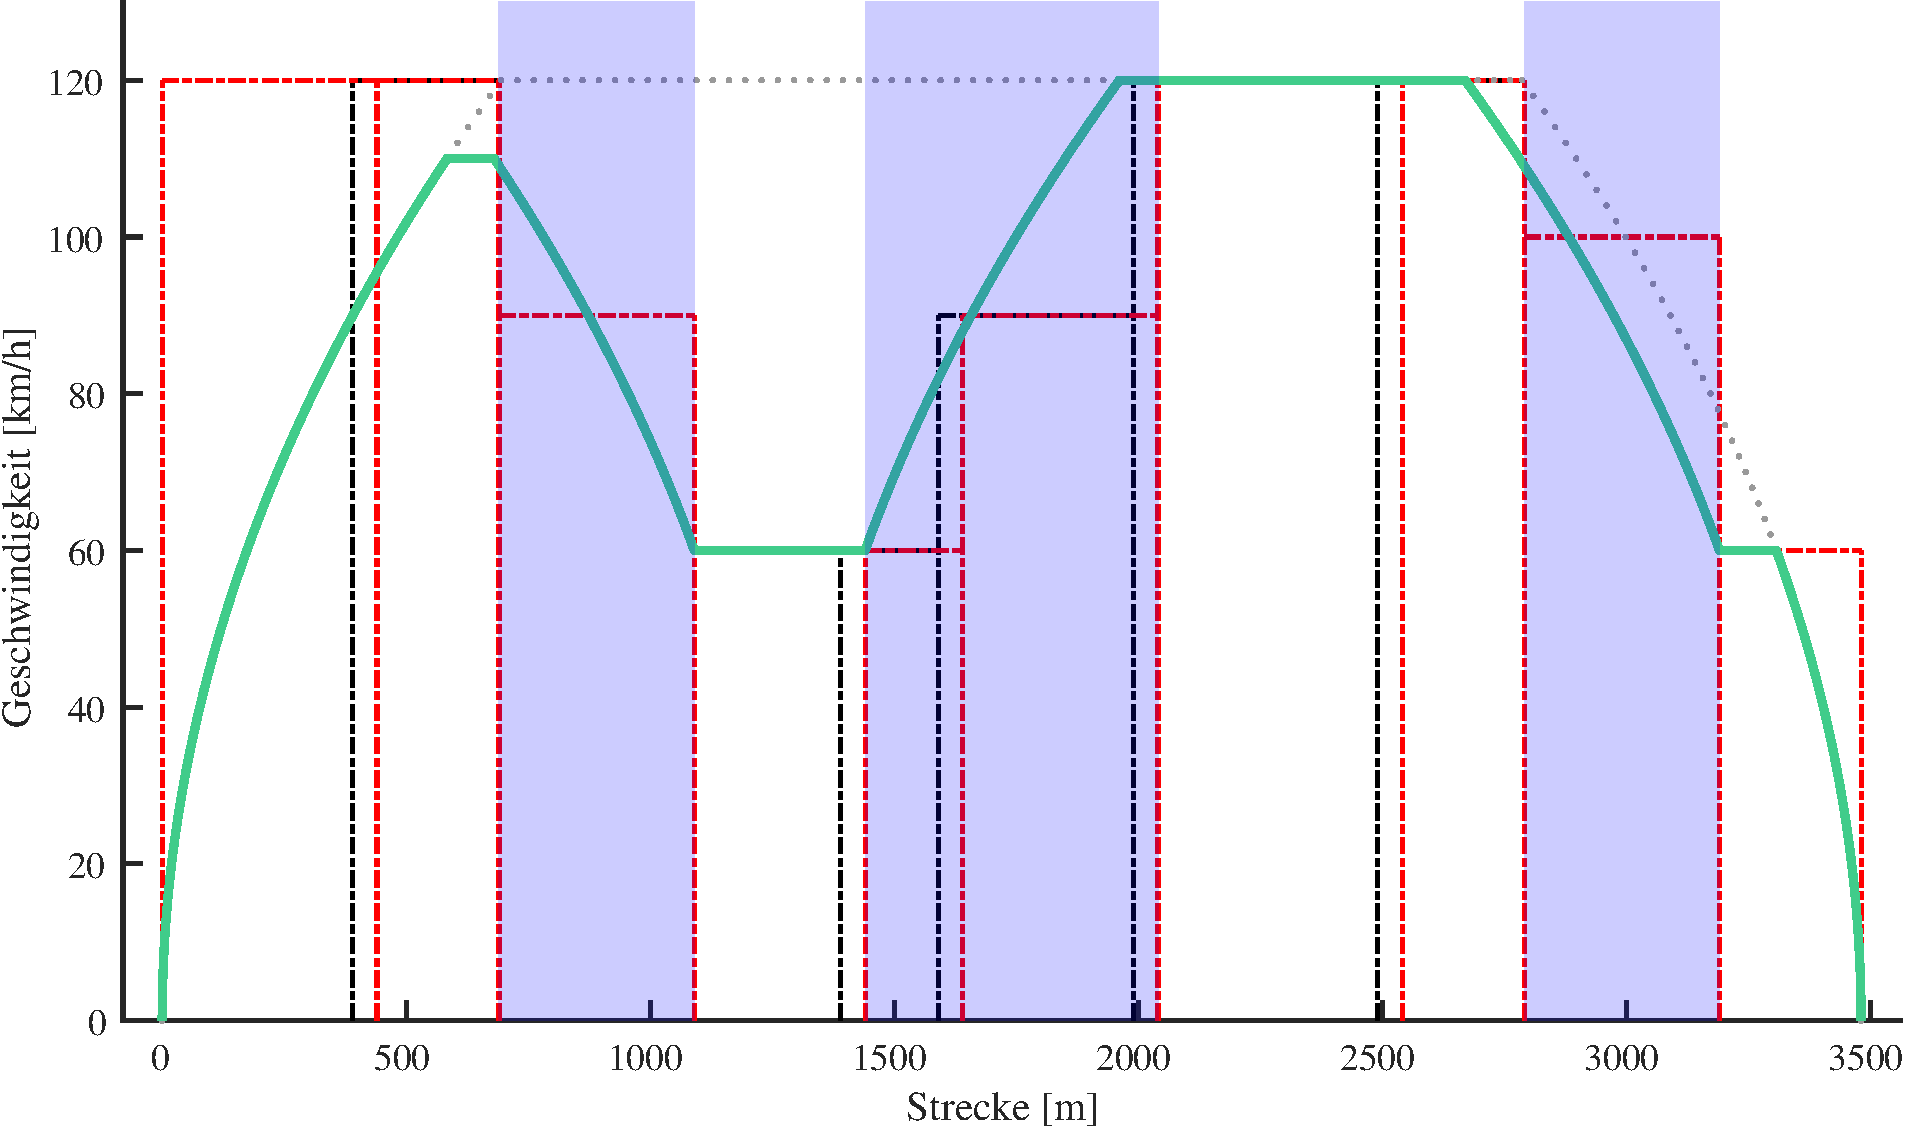
\includegraphics[width=\linewidth]{../matlab/it4.pdf}
  \caption{Fahrtverlaufberechnung (2. Iteration)}
  \label{fig:it4}
\end{figure}

\begin{figure}
  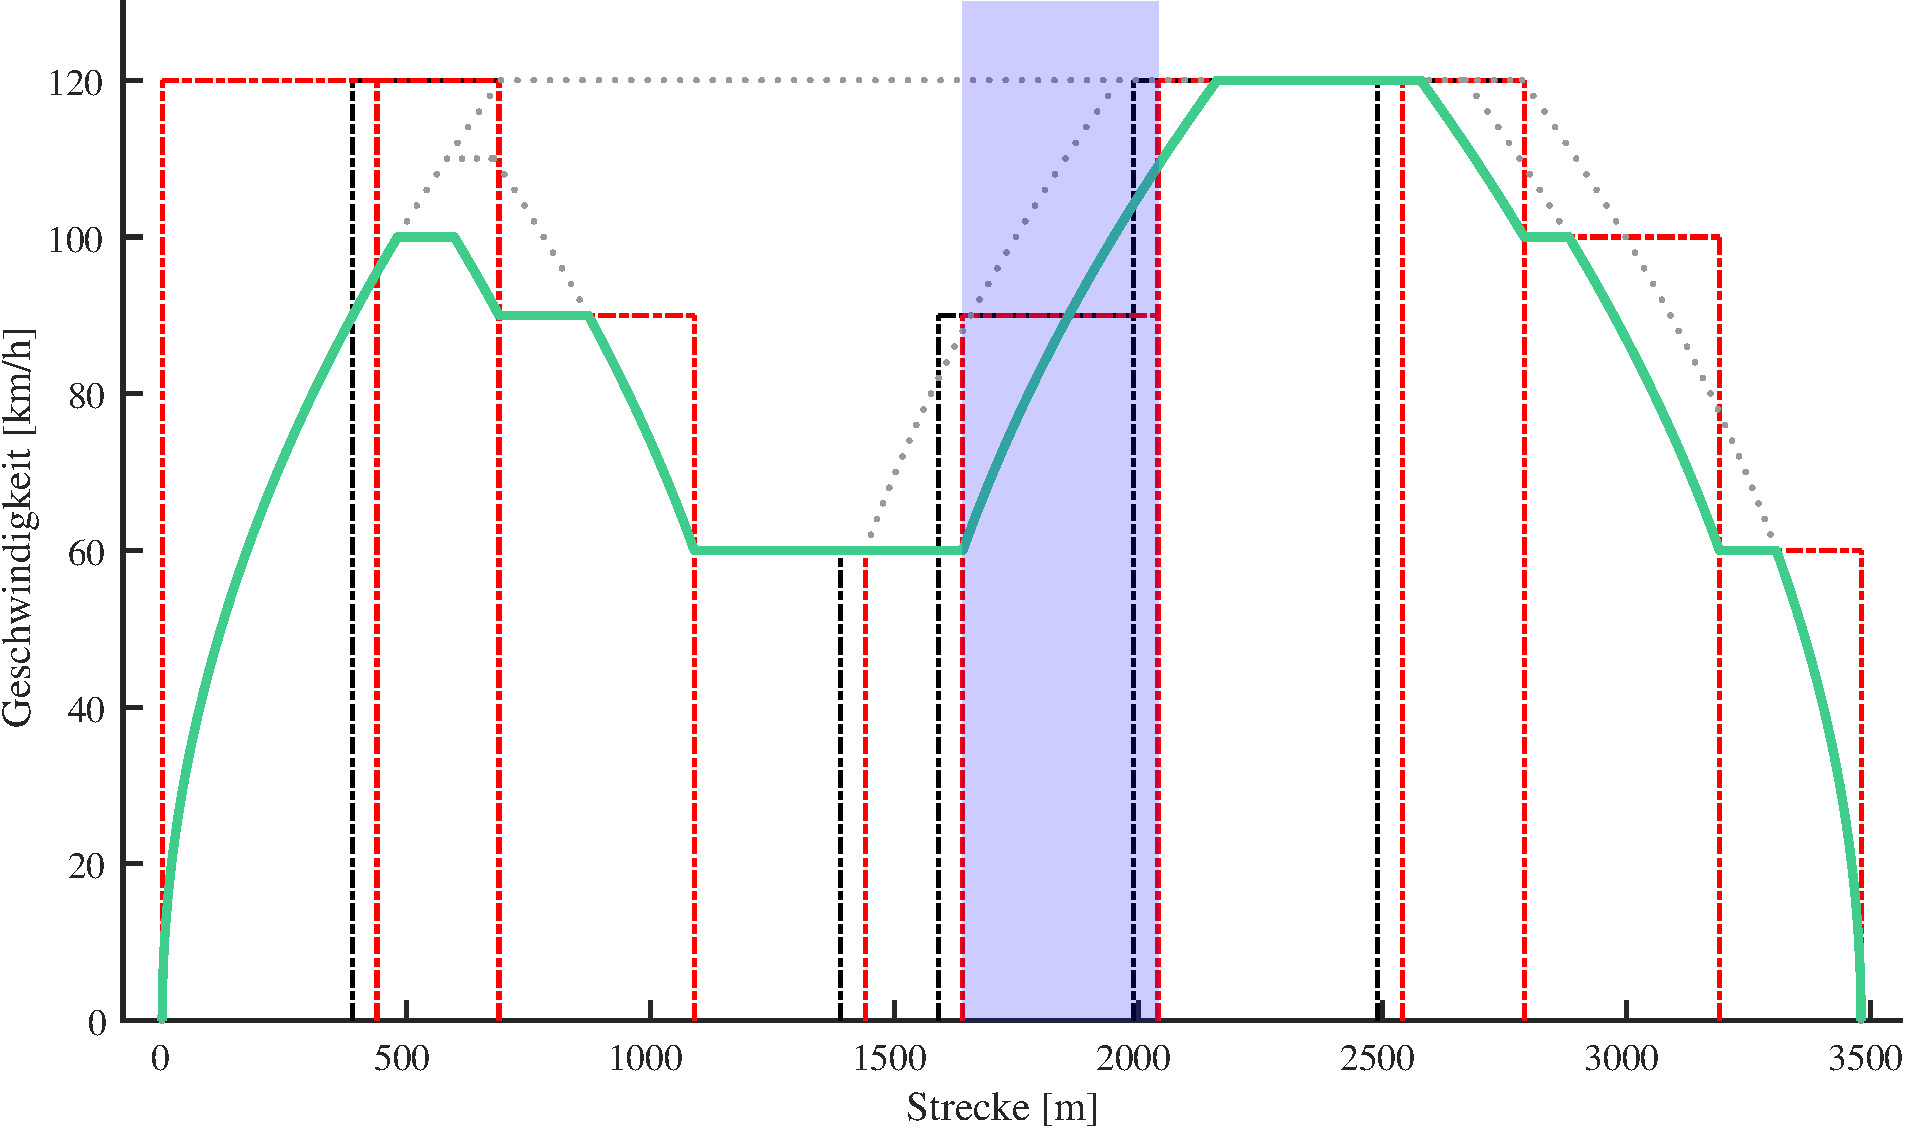
\includegraphics[width=\linewidth]{../matlab/it5.pdf}
  \caption{Fahrtverlaufberechnung (3. Iteration)}
  \label{fig:it5}
\end{figure}

\begin{figure}
  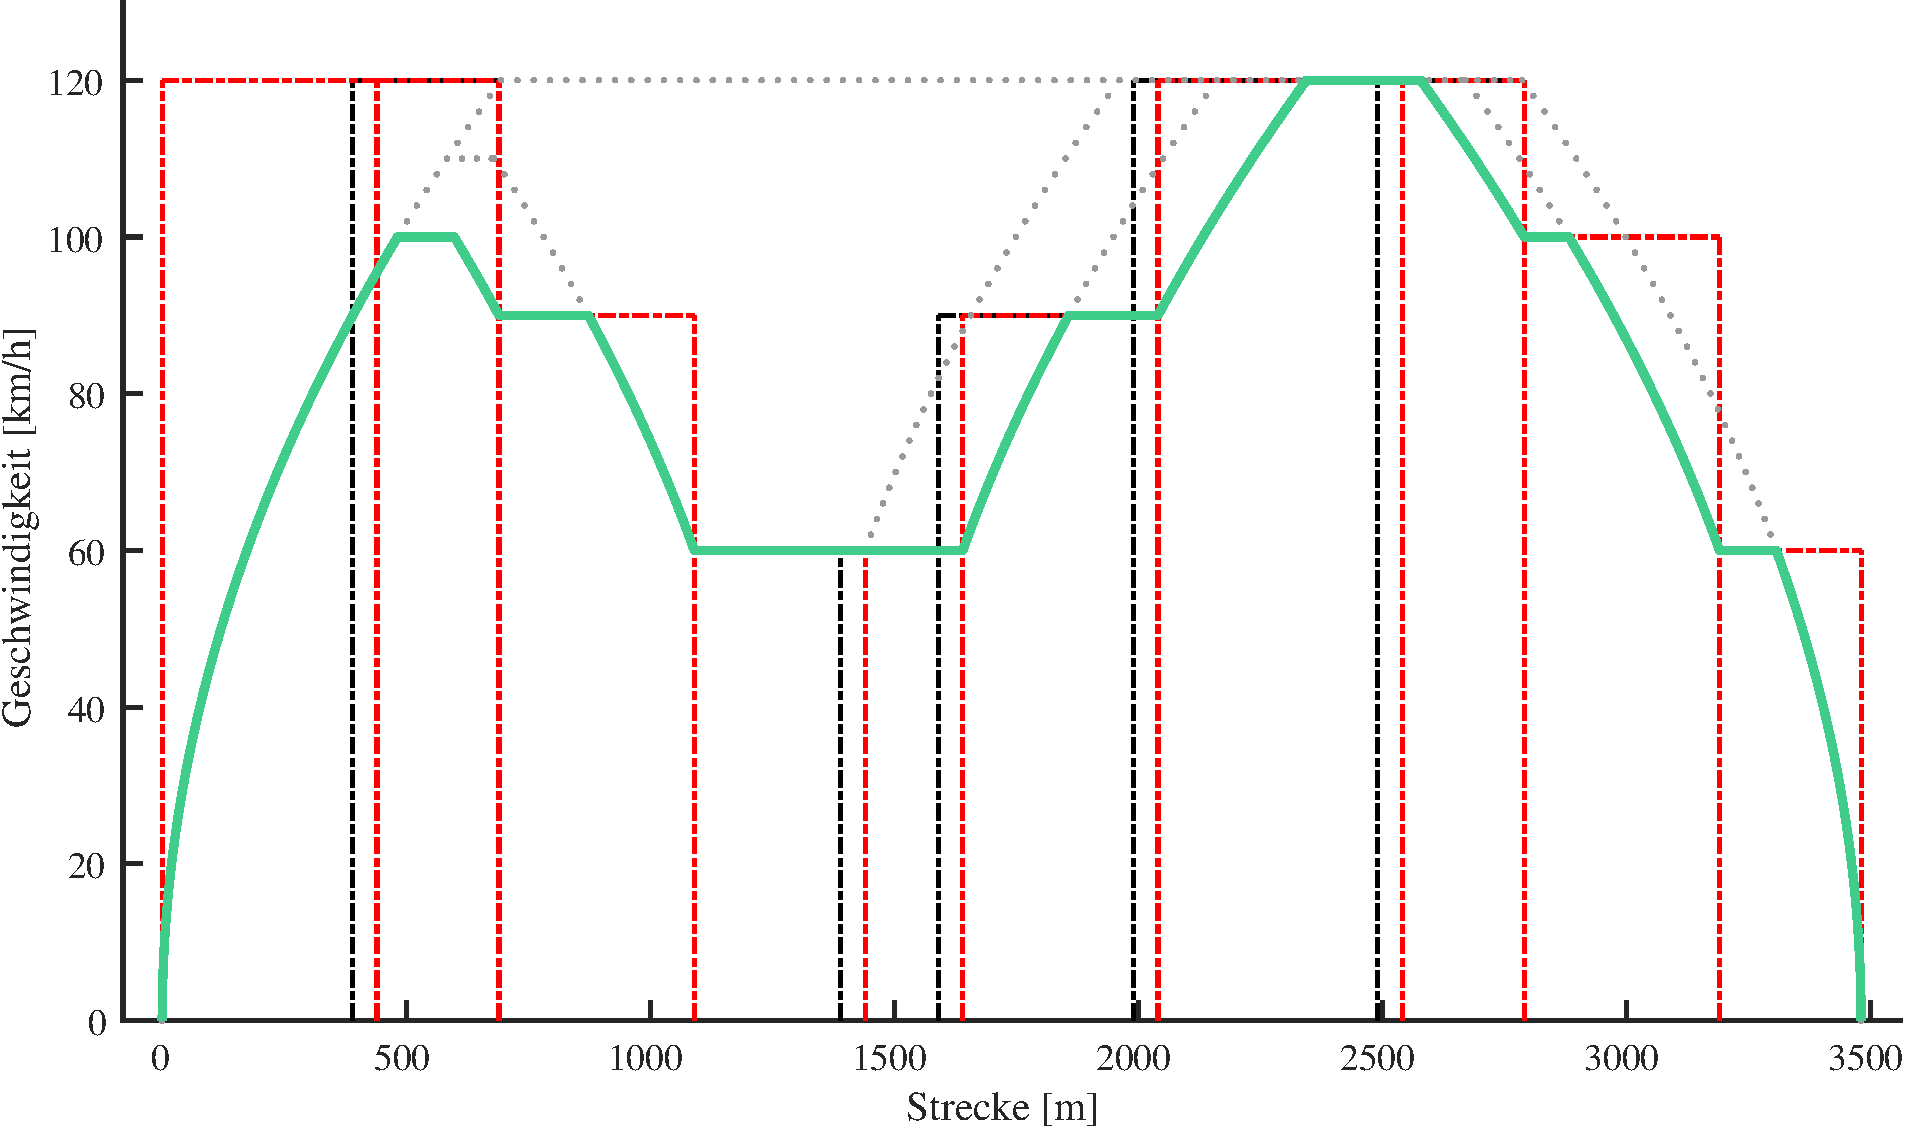
\includegraphics[width=\linewidth]{../matlab/it6.pdf}
  \caption{Fahrtverlaufberechnung (4. Iteration)}
  \label{fig:it6}
\end{figure}

\subsection{Einhaltung der Mindestzeit auf einer Geschwindigkeit} \label{minTime}

\begin{enumerate}
\item Ideal: möglichst späte v reduzieren
\end{enumerate}

Für eine möglichst realitätsnahe Simulation kann über die Variable \textit{\$globalTimeOnOneSpeed} in der Datei \textit{globalVariables.php} eine Mindestzeit festgelegt werden, die ein Fahrzeug auf einer Geschwindigkeit mindestens einhalten muss. Ebenfalls kann über die Variablen \textit{\$useMinTimeOnSpeed} und \textit{\$errorMinTimeOnSpeed} festgelegt werden, ob die Funktion aktiviert sein soll und ob es in dem Fall, dass diese Zeit nicht eingehalten werden kann, zu einer Fehlermeldung kommen soll. Im Falle einer Fehlermeldung würde das Fahrzeug nicht losfahren bzw. eine Gefahrenbremsung einleiten, falls das Fahrzeug aktuell eine Geschwindigkeit $v > 0$ hat. 

Wenn auf einem Abschnitt die Mindestzeit nicht eingehalten werden kann, kann eine Beschleunigung später eingeleitet werden, eine Verzögerung vorzeitiger eingeleitet werden oder auf eine kleinere Geschwindigkeit beschleunigt werden. In dem folgenden Algorithmus werden die \dots

Dadurch, dass sich eine Verschiebung einer Beschleunigung bzw. Verzögerung auf die nächsten Abschnitte auswirken kann, wird der Fahrtverlauf in \textit{\$subsections} unterteilt. Eine \textit{\$subsection} beschreibt dabei den Bereich des Fahrtverlaufs, in dem das Fahrzeug zum ersten Mal beschleunigt und zum letzten Mal abbremst. In der Darstellung \ref{fig:it7} wurde der exemplarische Fahrtverlauf somit in zwei \textit{\$subsection} unterteilt, welche Lila bzw. Gelb hinterlegt sind.
\begin{figure}
  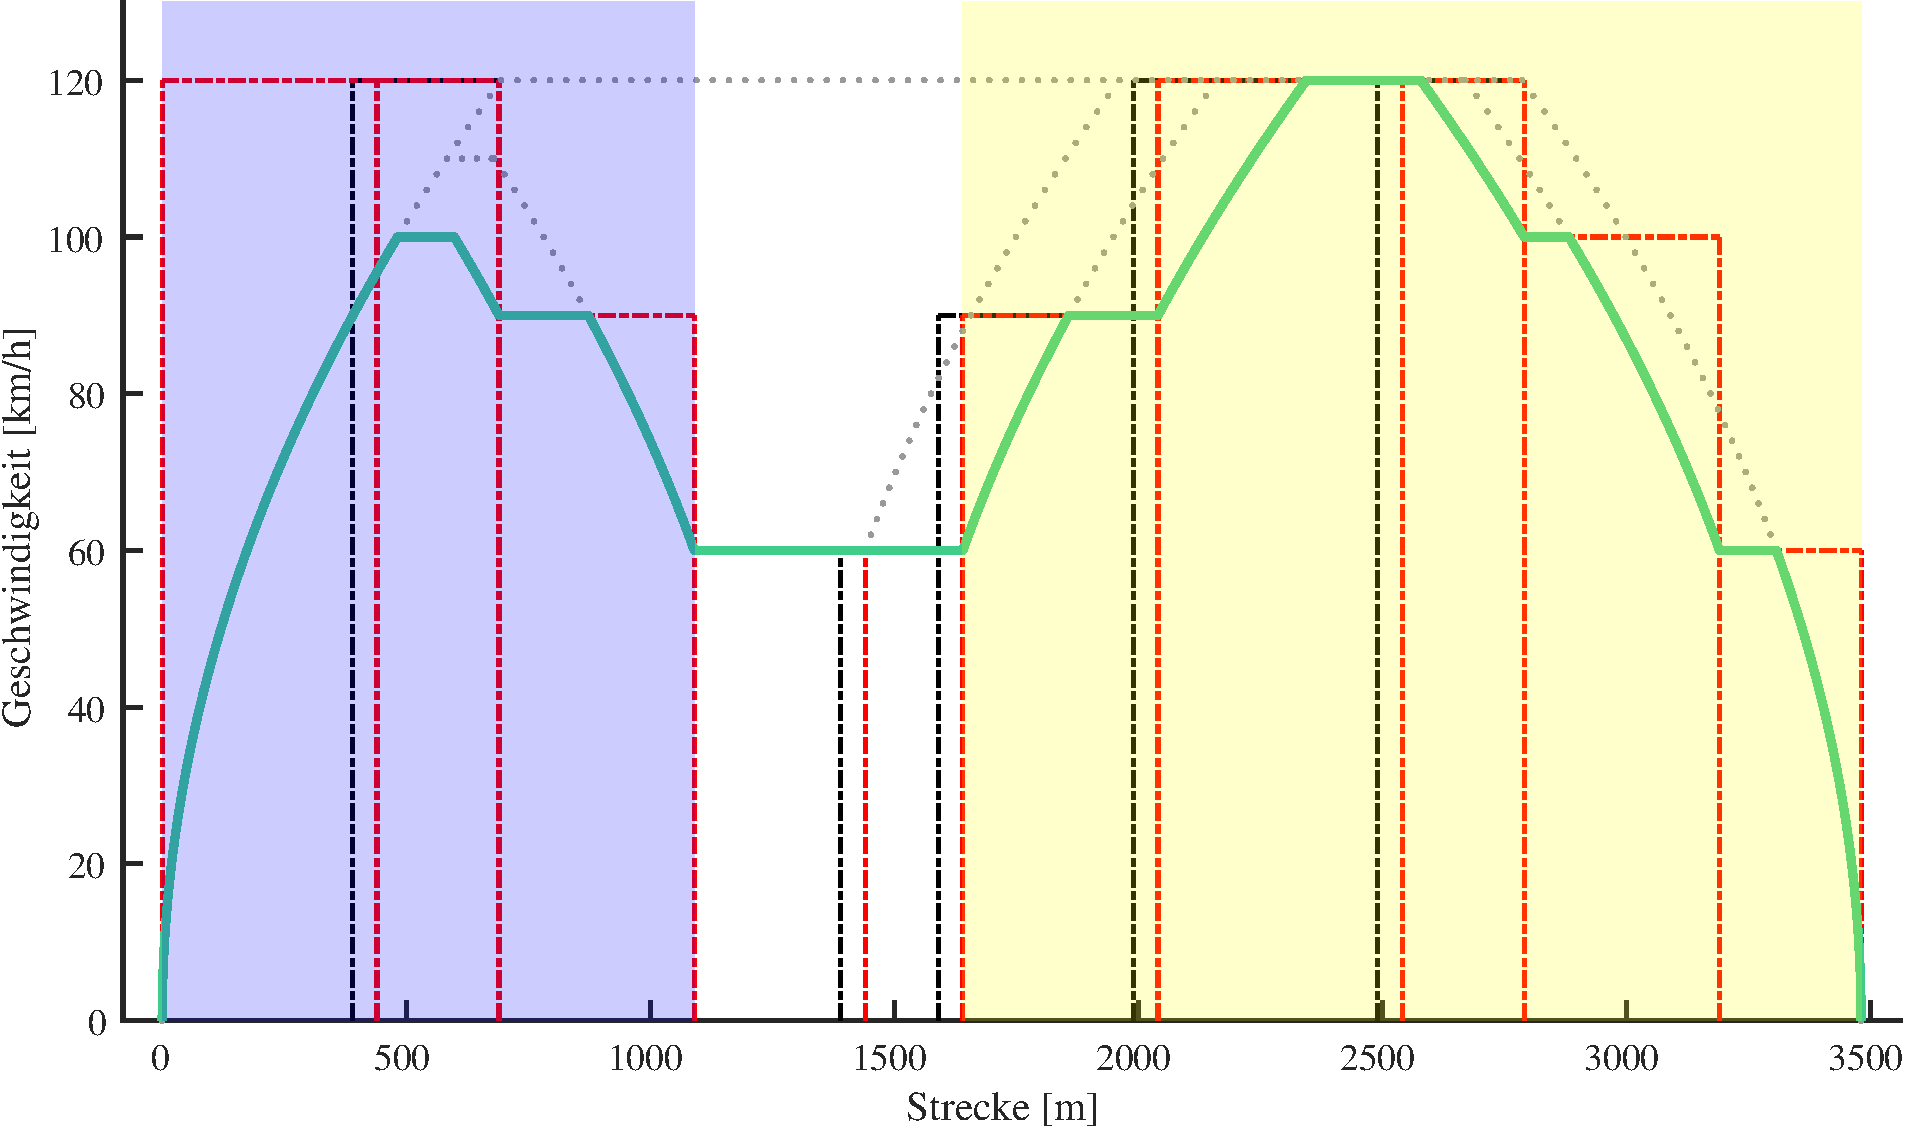
\includegraphics[width=\linewidth]{../matlab/it7.pdf}
  \caption{Einteilung des Fahrtverlaufs in \textit{\$subsections}}
  \label{fig:it7}
\end{figure}
Diese Einteilung wird vorgenommen, da sich die Verschiebung einer Beschleunigung bzw. Verzögerung auf die folgenden bzw. vorherigen Abschnitte auswirkt. Durch diese Einteilung kann verhindert werden, dass es dadurch zu Konflikten kommt. Falls die Beschleunigungen bzw. Verzögerungen soweit nach hinten bzw. nach vorne verschoben werden müssen, kann die maximale Geschwindigkeit auf dieser \textit{\$subsection} reduziert werden und die zur Verfügung stehende Strecke vergrößert werden. Wie in Darstellung \ref{fig:it7} zu erkennen wird hierbei im ersten Schritt der Abschnitt zwischen zwei \textit{\$subsections} ausgelassen. Nach der Ermittlung der \textit{subsections} wird überprüft, ob auf den Abschnitten zwischen den \textit{\$subsections} die Mindestzeit eingehalten wird. Wenn das nicht der Fall ist, wird der Abschnitt automatisch dem in Fahrtrichtung hinteren \textit{\$subsection} zugeordnet. Dadurch wird sichergestellt, dass das Fahrzeug, wenn es an einer Stelle des Fahrtbverlaufs die Geschwindigkeit reduziert, dies möglichst spät tut.

Nachdem die \textit{\$subsections} mittels der Funktion \textit{createSubsections$($$)$} erstellt wurden und mit der Funktion \textit{array\_reverse$($$)$} in umgekerte Reihenfolge in dem Array \textit{\$subsection\_list} gesammelt wurden, wird für jede \textit{\$subsection} überprüft, ob die Beschleunigungen bzw. Verzögerungen verschoben werden können. Dabei wird über alle konstanten Geschwindigkeiten iteriert, überprüft, ob die Mindestzeit eingehalten wird und wenn das nicht der Fall ist, wird überprüft, ob eine Verschiebung möglich ist. Sollte bei einer Verschiebung die $position\_1$ des \textit{\$keyPoints} hinter $position\_0$ des zweiten \textit{\$keyPoints} liegen (bei einer Beschleunigung), wird der zweite \textit{\$keyPoint} gelöscht. Gleiches geschieht bei der Verzögerung in umgekehrter Reihenfolge. Nach der Verschiebung wird überprüft, ob auf allen konstanten Geschwindigkeit die Mindestzeit eingehalten wird. Wenn das der Fall ist, wird die nächste \textit{\$subsection} überprüft. In dem Fall, dass durch die Verschiebung die Mindestueit nicht eingehalten werden kann, wird die maximale Geschcindigkeit auf dieser \textit{\$subsection} um $10 km/h$ reduziert, die \textit{\$subsections} neu berechnet und erneut über alle \textit{\$subsection} iteriert. Die Neuberechnung ist notwendig, da durch die Reduzierung der Geschwindigkeit die \textit{\$subsections} anders aufgeteilt sein können.

Wenn alle \textit{\$subsections} die Mindestzeit einhalten, wird der Algorithmus beendet. In der Darstellung \ref{fig:it9} ist der Fahrtverlauf unter Einhaltung der Mindestzeit auf einer Geschwindigkeit abgebildet.
\begin{enumerate}
\item $v_0 not equal 0 km/h$
\item Überprüfung, ob es überhaupt möglich ist.
\end{enumerate}
\begin{figure}
  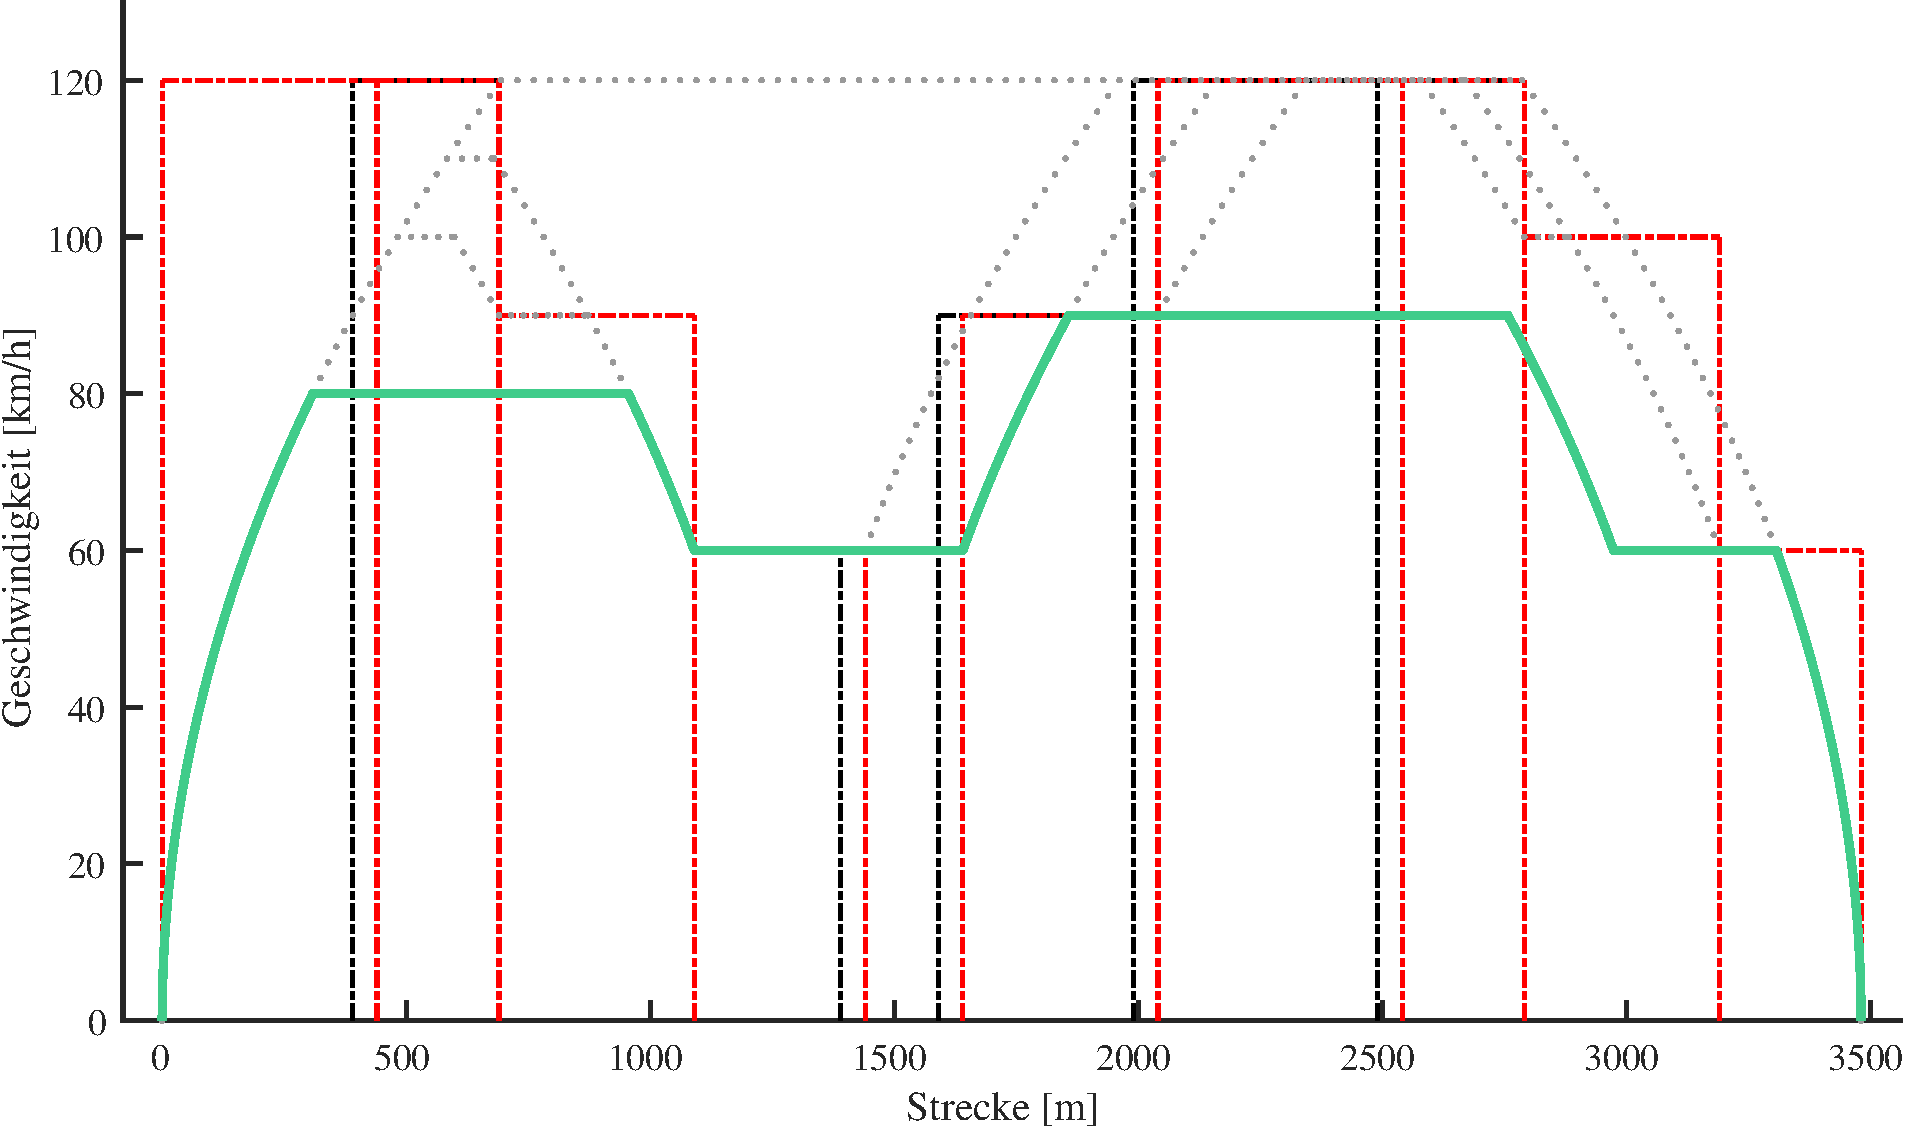
\includegraphics[width=\linewidth]{../matlab/it9.pdf}
  \caption{Fahrtverlauf unter Einhaltung der Mindestzeit}
  \label{fig:it9}
\end{figure}
\begin{table}
\begin{center}
\renewcommand{\arraystretch}{1.2}
\begin{tabular}{c|c}
Index & Funktion \\ \hline
\textit{max\_index}                 &   \makecell{ndex des \textit{\$keyPoints} mit der Beschleunigung auf die\\maximale Geschwindigkeit in der \textit{\$subsection}}     \\ \hline
\textit{indexes}                 &    Indexe aller beinhalteten \textit{\$keyPoints}                  \\ \hline
\textit{is\_prev\_section}              &   Berücksichtigung des Abschnitts vor der \textit{\$subsection}     \\ \hline
\textit{is\_next\_section}                 &     Berücksichtigung des Abschnitts nach der \textit{\$subsection}                 \\ \hline
\textit{failed}                 &   Unterschreitung der Mindestzeit auf der \textit{\$subsection}     \\ \hline
\textit{brakes\_only}                    &   \textit{\dots\dots}                  \\
\end{tabular}
\renewcommand{\arraystretch}{1}
\caption{Aufbau des \textit{\$subsection}-Arrays}
\label{table:subsection}
\end{center}
\end{table}
Für den Fall, dass das Fahrzeug auf einer Geschwindigkeit die Mindestzeit nicht einhält und als nächstes beschleunigen würde, kann die Beschleunigung später eingeleitet werden. 
\subsection{Berücksichtigung der Ankunfrtszeit bei der Berechnung des Fahrtverlaufs} \label{time}
Der berechnete Fahrtverlauf in Kapitel \ref{v_max}, \ref{überprüfung}, \ref{neuberechnung} und \ref{minTime} ermittelt die frühstmögliche Ankunftszeit am Ziel. In dem Fall, dass der Zug dadurch mit einer Verspätung am Ziel ankommt wird der Fahrtverlauf an das Fahrzeug übergeben. Falls der Zug allerdings mit dem Fahrtverlauf zu früh am Ziel ankommen würde, wird überprüft, ob es möglich ist die Geschwindigkeit zu reduzieren, sodass der Zug energieeffizienter fahren kann und ohne Verspätung am Ziel ankommt.

Ergebnis ist in \ref{fig:it10} abgebildet.

NACHSCHAUEN, WAS DER ALGORITHMUS GENAU MACHT!

\begin{figure}
  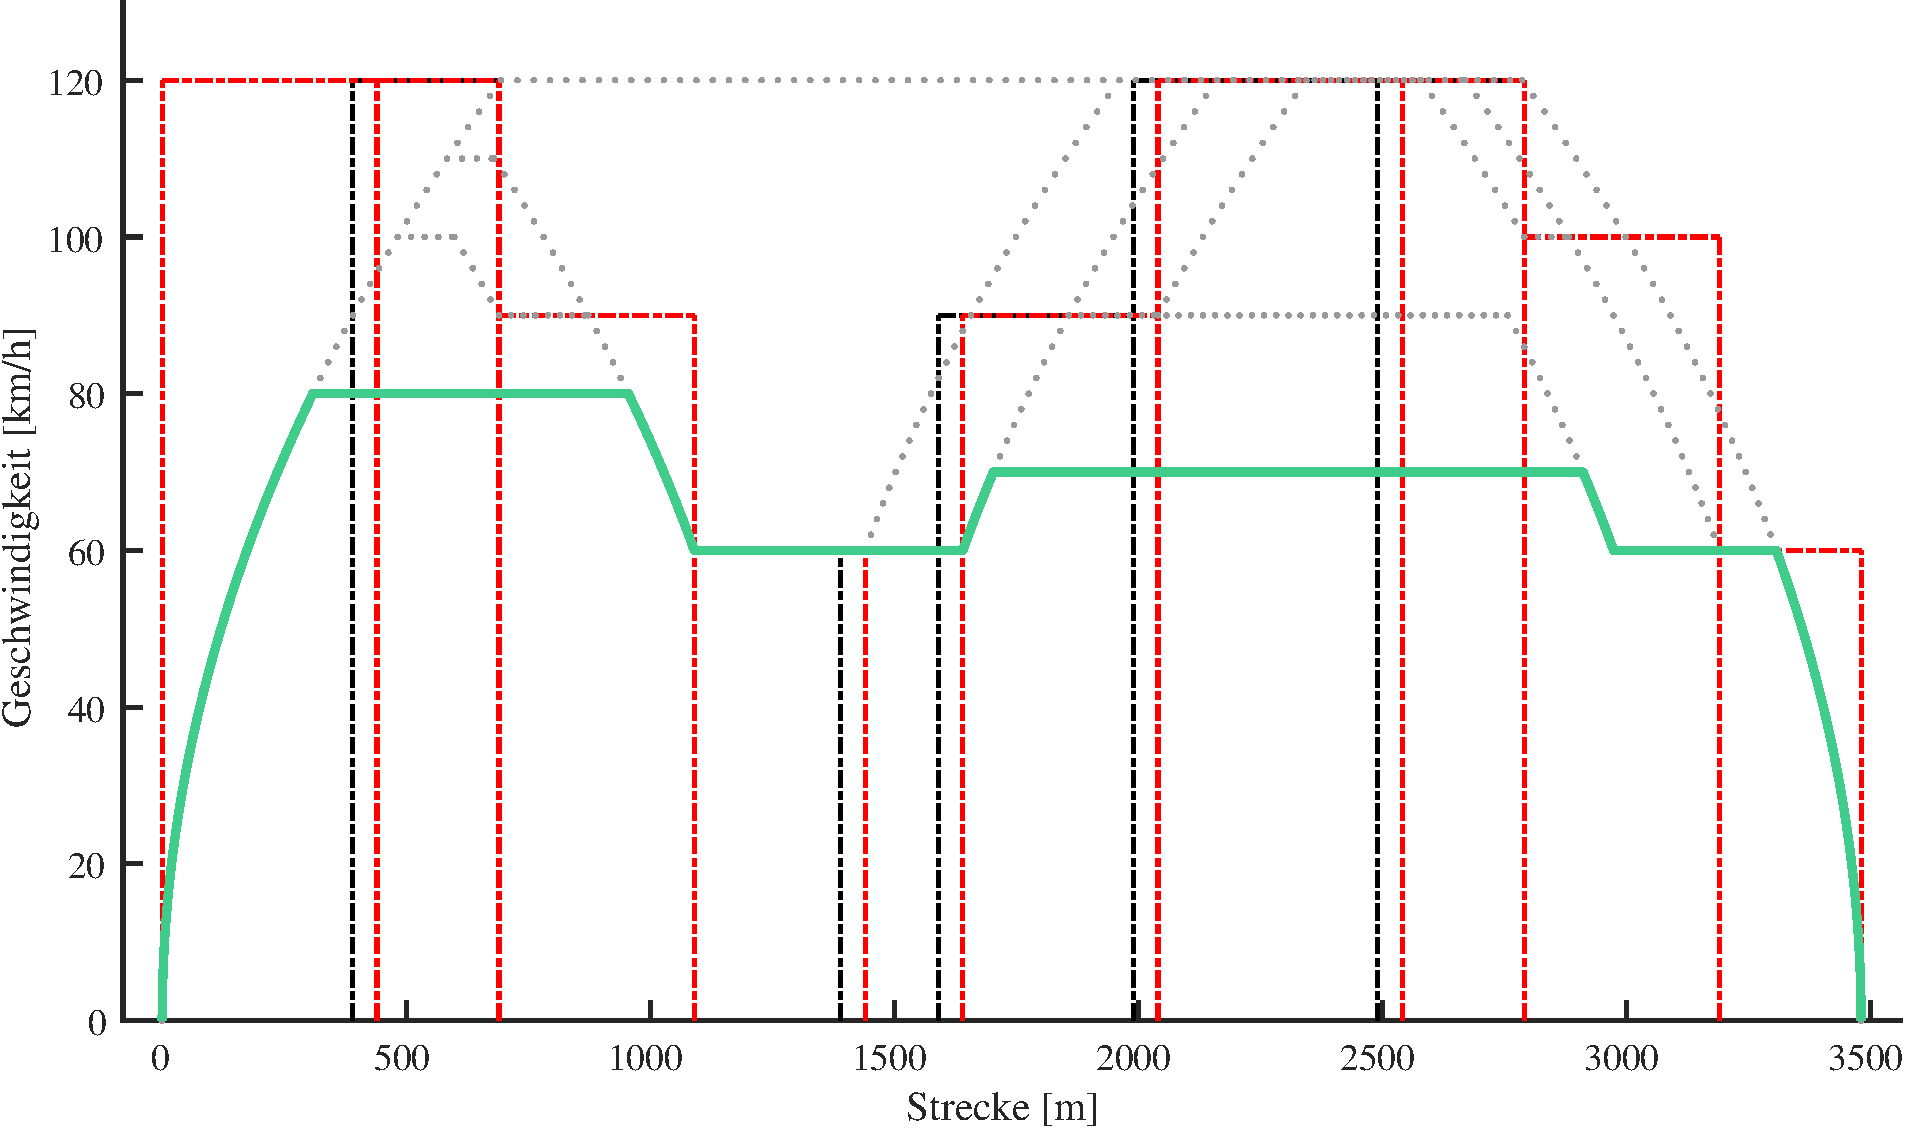
\includegraphics[width=\linewidth]{../matlab/it10.pdf}
  \caption{Fahrtverlauf mit reduzierter Geschwindigkeit unter Einhaltung der Ankunftszeit}
  \label{fig:it10}
\end{figure}


\subsection{Berücksichtigung der exakten Ankunfrtszeit bei der Berechnung des Fahrtverlaufs} \label{time2}

Die in Kapitel \ref{minTime} errechnete Ankunftszeit, beschreibt die spätmöglichste Ankunftszueit am Ziel, ohne dass das Fahrzeug mit einer Verspätung am Ziel ankommt, wenn bei einer Beschleunigung auf eine geringere Zielgeschwindigkeit beschleunigt wird. Dadurch wird das Fahrzeug im Normalfall noch nicht exakt pünktlich das Ziel erreichen. Über die Variable \textit{\$useSpeedFineTuning} kann festgelegt werden, ob das Fahrzeug eine exakte Ankunftsazeit versuchen soll zu erreichen. 

Wenn diese Funktion aktiviert ist, wird versucht die vorletzten Verzögerung vorzeitiger einzuleiten. Für den Fall, dass es auf dem gesamten Fahrtverlauf nur eine Verzögerung gibt, wird überprüft, ob das Fahrzeug anstatt der einen Verzögerung erst auf $10 km/h$ abbremsen kann und und kurz vorm Ziel von $10 km/h$ auf $0 km/h$ abbremsen kann.



\begin{figure}
  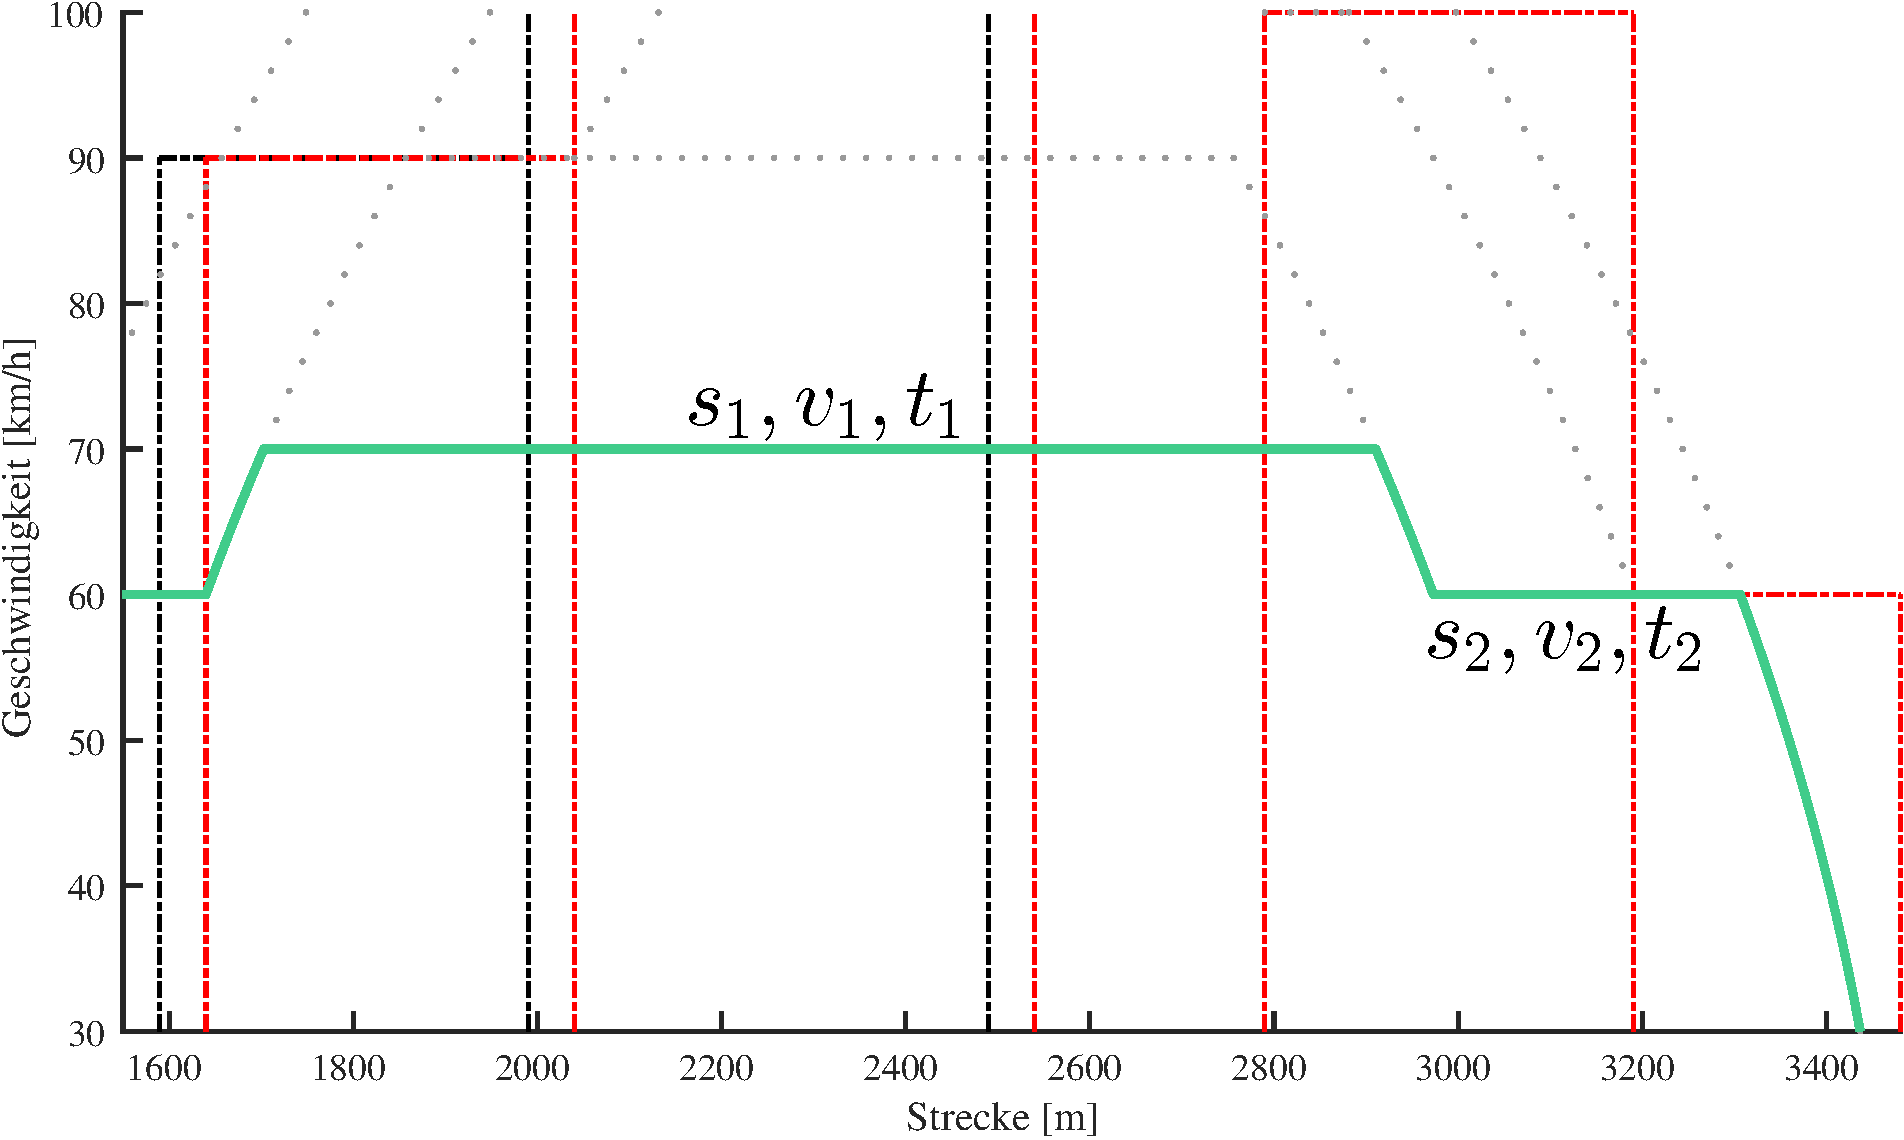
\includegraphics[width=\linewidth]{../matlab/it11.pdf}
  \caption{speedFineTuning\_1}
  \label{fig:it11}
\end{figure}
\begin{figure}
  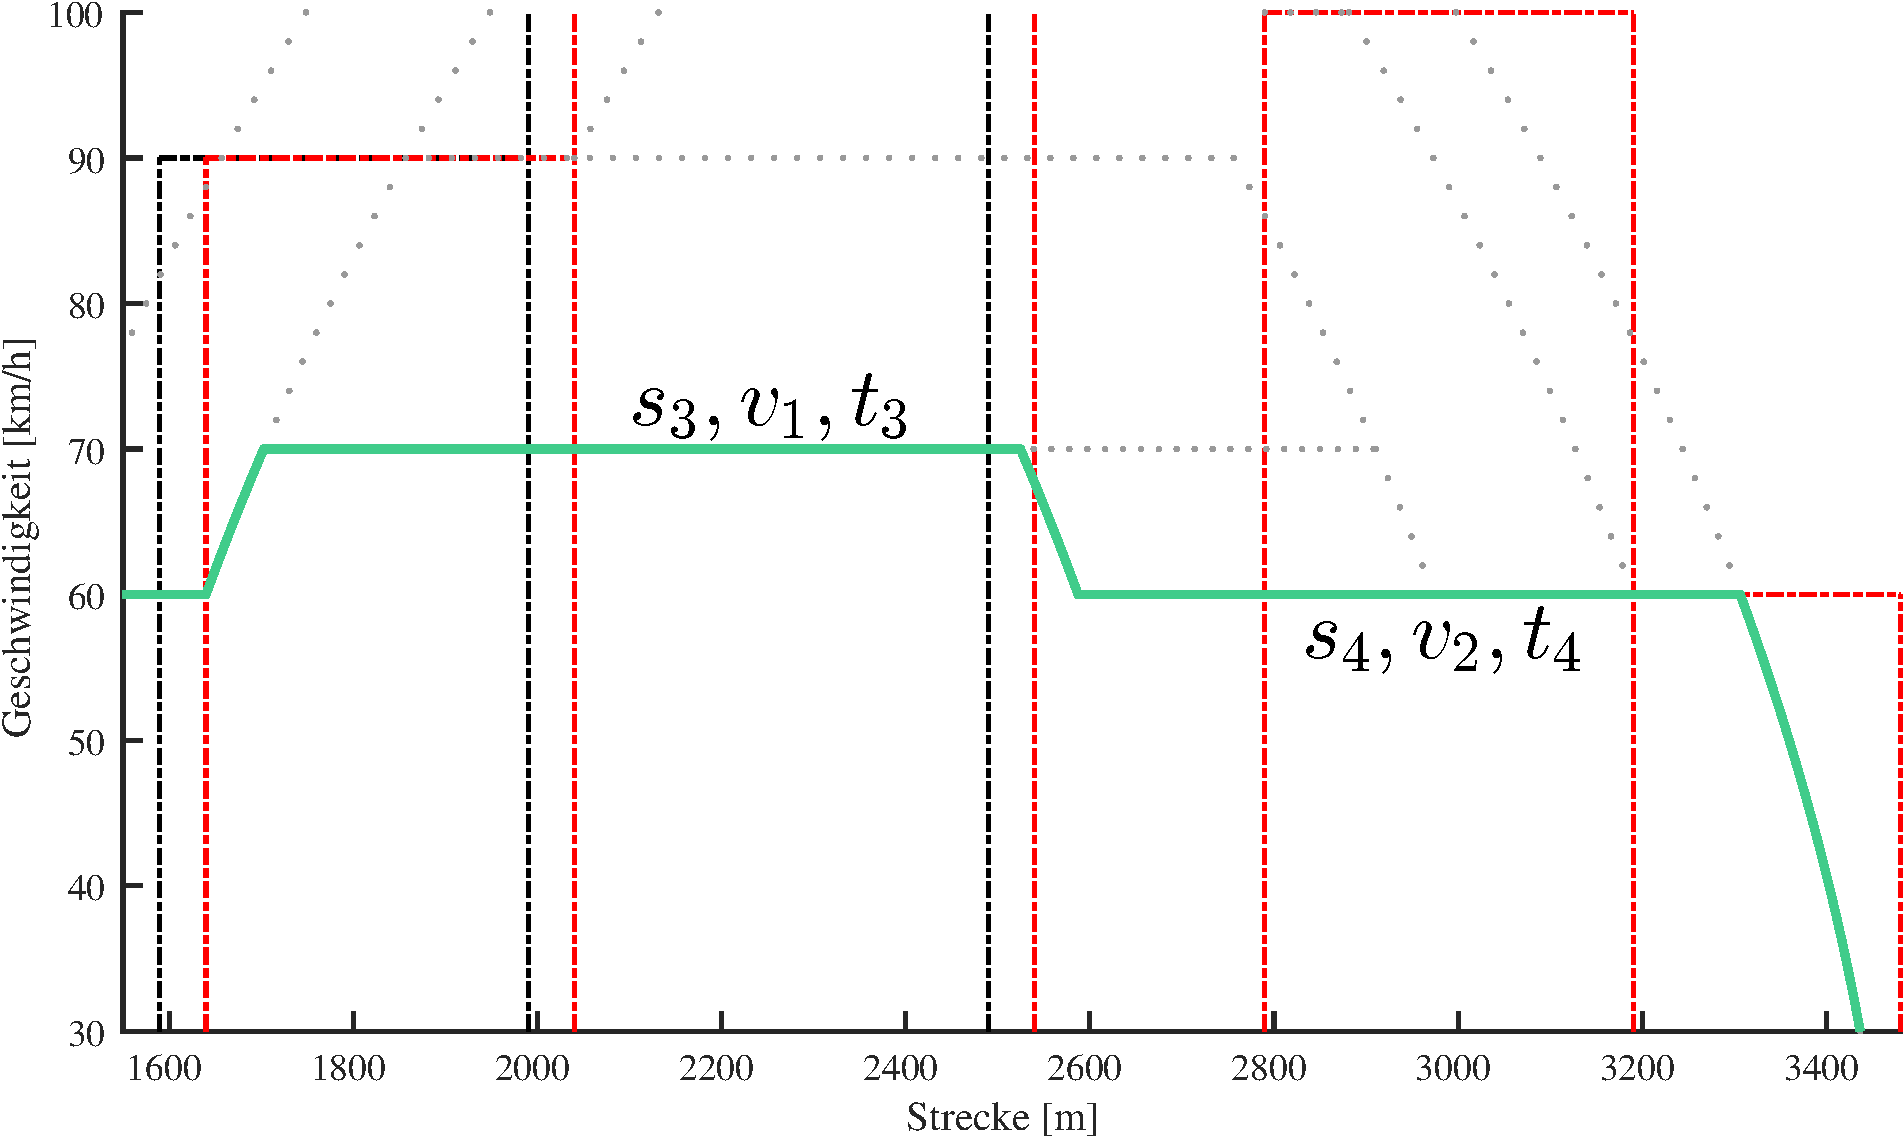
\includegraphics[width=\linewidth]{../matlab/it12.pdf}
  \caption{speedFineTuning\_2}
  \label{fig:it12}
\end{figure}
\begin{figure}
  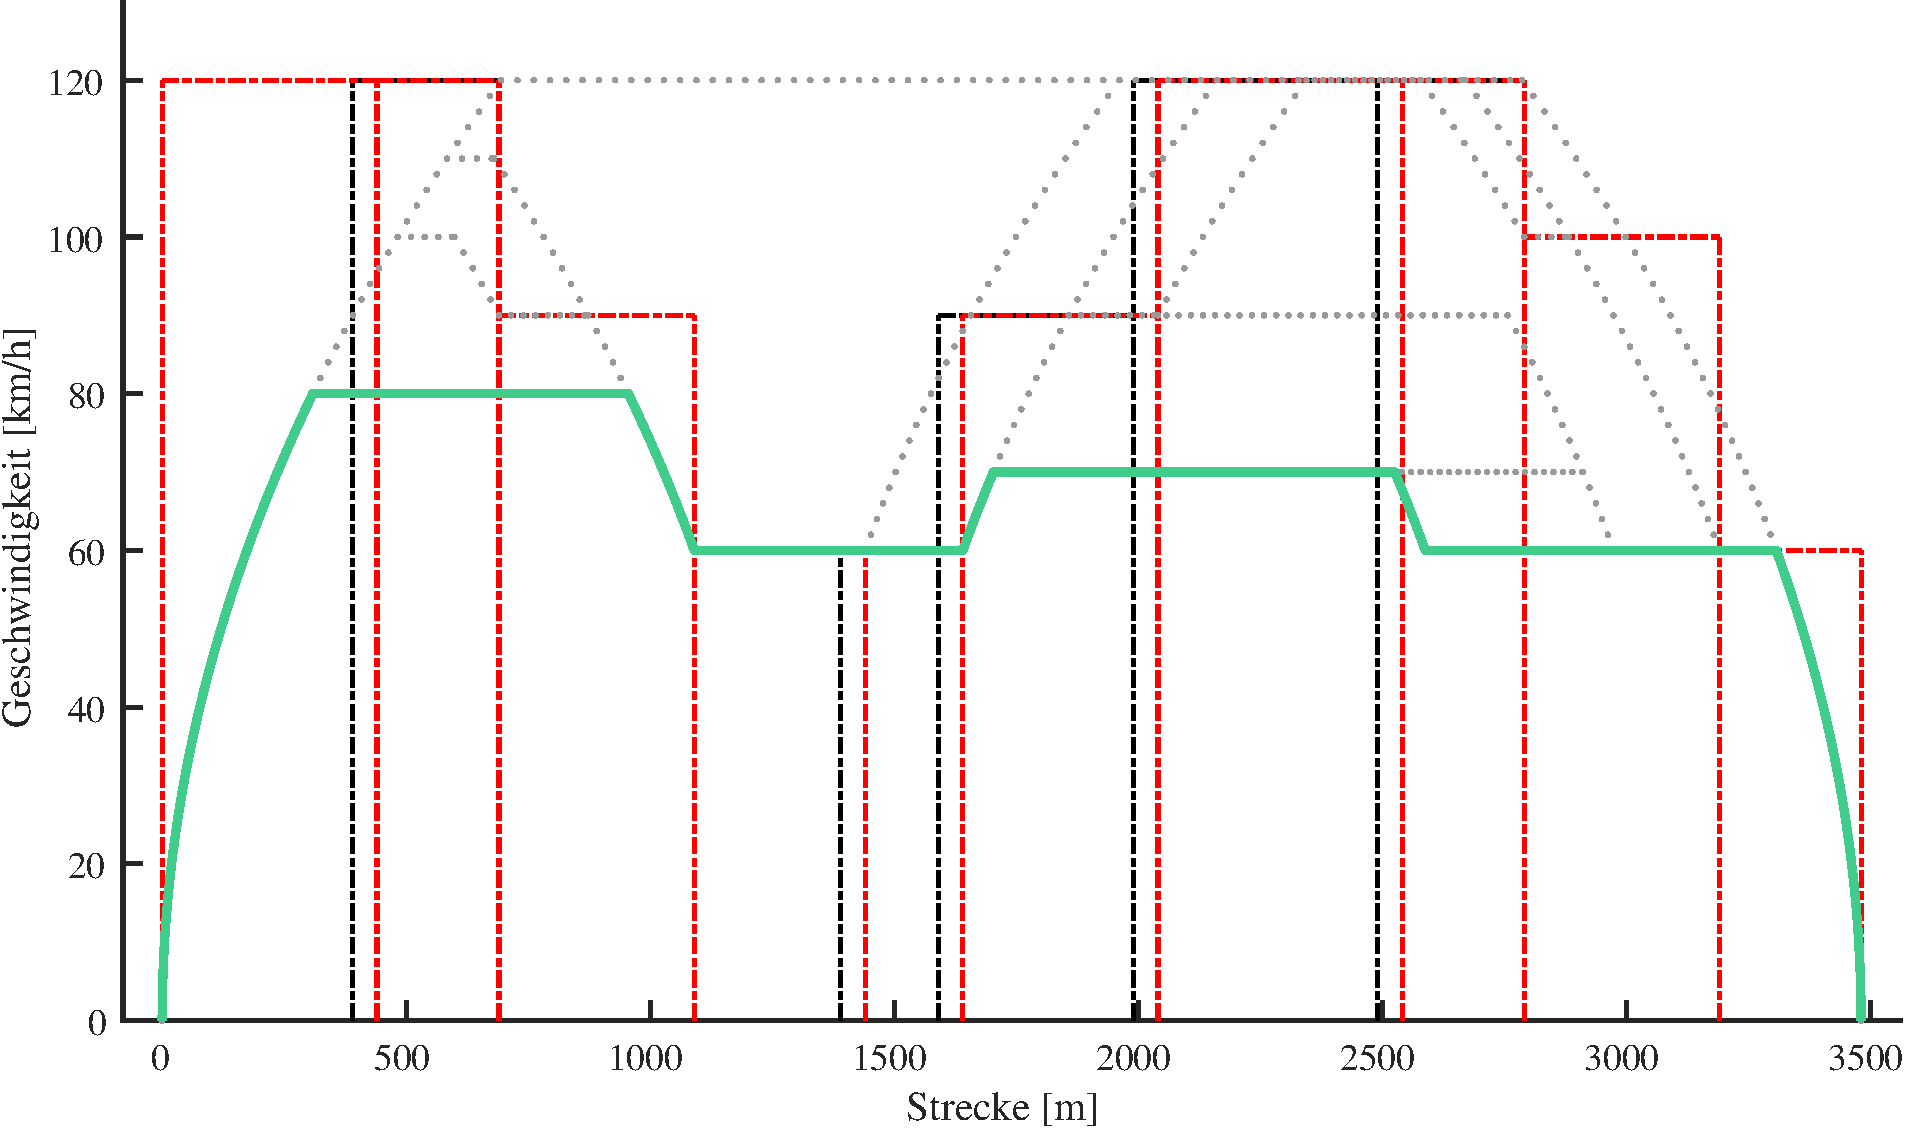
\includegraphics[width=\linewidth]{../matlab/it13.pdf}
  \caption{Finaler Fahrtverlauf}
  \label{fig:it13}
\end{figure}

\subsection{Einleitung einer Gefahrenbremsung} \label{notbremsung}




































